\documentclass[twoside]{book}

% Packages required by doxygen
\usepackage{fixltx2e}
\usepackage{calc}
\usepackage{doxygen}
\usepackage[export]{adjustbox} % also loads graphicx
\usepackage{graphicx}
\usepackage[utf8]{inputenc}
\usepackage{makeidx}
\usepackage{multicol}
\usepackage{multirow}
\PassOptionsToPackage{warn}{textcomp}
\usepackage{textcomp}
\usepackage[nointegrals]{wasysym}
\usepackage[table]{xcolor}

% Font selection
\usepackage[T1]{fontenc}
\usepackage[scaled=.90]{helvet}
\usepackage{courier}
\usepackage{amssymb}
\usepackage{sectsty}
\renewcommand{\familydefault}{\sfdefault}
\allsectionsfont{%
  \fontseries{bc}\selectfont%
  \color{darkgray}%
}
\renewcommand{\DoxyLabelFont}{%
  \fontseries{bc}\selectfont%
  \color{darkgray}%
}
\newcommand{\+}{\discretionary{\mbox{\scriptsize$\hookleftarrow$}}{}{}}

% Page & text layout
\usepackage{geometry}
\geometry{%
  a4paper,%
  top=2.5cm,%
  bottom=2.5cm,%
  left=2.5cm,%
  right=2.5cm%
}
\tolerance=750
\hfuzz=15pt
\hbadness=750
\setlength{\emergencystretch}{15pt}
\setlength{\parindent}{0cm}
\setlength{\parskip}{3ex plus 2ex minus 2ex}
\makeatletter
\renewcommand{\paragraph}{%
  \@startsection{paragraph}{4}{0ex}{-1.0ex}{1.0ex}{%
    \normalfont\normalsize\bfseries\SS@parafont%
  }%
}
\renewcommand{\subparagraph}{%
  \@startsection{subparagraph}{5}{0ex}{-1.0ex}{1.0ex}{%
    \normalfont\normalsize\bfseries\SS@subparafont%
  }%
}
\makeatother

% Headers & footers
\usepackage{fancyhdr}
\pagestyle{fancyplain}
\fancyhead[LE]{\fancyplain{}{\bfseries\thepage}}
\fancyhead[CE]{\fancyplain{}{}}
\fancyhead[RE]{\fancyplain{}{\bfseries\leftmark}}
\fancyhead[LO]{\fancyplain{}{\bfseries\rightmark}}
\fancyhead[CO]{\fancyplain{}{}}
\fancyhead[RO]{\fancyplain{}{\bfseries\thepage}}
\fancyfoot[LE]{\fancyplain{}{}}
\fancyfoot[CE]{\fancyplain{}{}}
\fancyfoot[RE]{\fancyplain{}{\bfseries\scriptsize Generated by Doxygen }}
\fancyfoot[LO]{\fancyplain{}{\bfseries\scriptsize Generated by Doxygen }}
\fancyfoot[CO]{\fancyplain{}{}}
\fancyfoot[RO]{\fancyplain{}{}}
\renewcommand{\footrulewidth}{0.4pt}
\renewcommand{\chaptermark}[1]{%
  \markboth{#1}{}%
}
\renewcommand{\sectionmark}[1]{%
  \markright{\thesection\ #1}%
}

% Indices & bibliography
\usepackage{natbib}
\usepackage[titles]{tocloft}
\setcounter{tocdepth}{3}
\setcounter{secnumdepth}{5}
\makeindex

% Hyperlinks (required, but should be loaded last)
\usepackage{ifpdf}
\ifpdf
  \usepackage[pdftex,pagebackref=true]{hyperref}
\else
  \usepackage[ps2pdf,pagebackref=true]{hyperref}
\fi
\hypersetup{%
  colorlinks=true,%
  linkcolor=blue,%
  citecolor=blue,%
  unicode%
}

% Custom commands
\newcommand{\clearemptydoublepage}{%
  \newpage{\pagestyle{empty}\cleardoublepage}%
}

\usepackage{caption}
\captionsetup{labelsep=space,justification=centering,font={bf},singlelinecheck=off,skip=4pt,position=top}

%===== C O N T E N T S =====

\begin{document}

% Titlepage & ToC
\hypersetup{pageanchor=false,
             bookmarksnumbered=true,
             pdfencoding=unicode
            }
\pagenumbering{alph}
\begin{titlepage}
\vspace*{7cm}
\begin{center}%
{\Large Lista5 }\\
\vspace*{1cm}
{\large Generated by Doxygen 1.8.14}\\
\end{center}
\end{titlepage}
\clearemptydoublepage
\pagenumbering{roman}
\tableofcontents
\clearemptydoublepage
\pagenumbering{arabic}
\hypersetup{pageanchor=true}

%--- Begin generated contents ---
\chapter{Namespace Index}
\section{Packages}
Here are the packages with brief descriptions (if available)\+:\begin{DoxyCompactList}
\item\contentsline{section}{\mbox{\hyperlink{namespacelista__5}{lista\+\_\+5}} }{\pageref{namespacelista__5}}{}
\end{DoxyCompactList}

\chapter{Hierarchical Index}
\section{Class Hierarchy}
This inheritance list is sorted roughly, but not completely, alphabetically\+:\begin{DoxyCompactList}
\item Float\begin{DoxyCompactList}
\item \contentsline{section}{lista\+\_\+5.\+Kolo}{\pageref{classlista__5_1_1_kolo}}{}
\end{DoxyCompactList}
\item Float\begin{DoxyCompactList}
\item \contentsline{section}{lista\+\_\+5.\+Prostokat}{\pageref{classlista__5_1_1_prostokat}}{}
\end{DoxyCompactList}
\item J\+Frame\begin{DoxyCompactList}
\item \contentsline{section}{lista\+\_\+5.\+Info}{\pageref{classlista__5_1_1_info}}{}
\item \contentsline{section}{lista\+\_\+5.\+Painty}{\pageref{classlista__5_1_1_painty}}{}
\end{DoxyCompactList}
\item J\+Popup\+Menu\begin{DoxyCompactList}
\item \contentsline{section}{lista\+\_\+5.\+Menu\+Kontekstowe}{\pageref{classlista__5_1_1_menu_kontekstowe}}{}
\end{DoxyCompactList}
\item Polygon\begin{DoxyCompactList}
\item \contentsline{section}{lista\+\_\+5.\+Wielokat}{\pageref{classlista__5_1_1_wielokat}}{}
\end{DoxyCompactList}
\item Shape\begin{DoxyCompactList}
\item \contentsline{section}{lista\+\_\+5.\+Figura}{\pageref{interfacelista__5_1_1_figura}}{}
\begin{DoxyCompactList}
\item \contentsline{section}{lista\+\_\+5.\+Kolo}{\pageref{classlista__5_1_1_kolo}}{}
\item \contentsline{section}{lista\+\_\+5.\+Prostokat}{\pageref{classlista__5_1_1_prostokat}}{}
\item \contentsline{section}{lista\+\_\+5.\+Wielokat}{\pageref{classlista__5_1_1_wielokat}}{}
\end{DoxyCompactList}
\end{DoxyCompactList}
\item Action\+Listener\begin{DoxyCompactList}
\item \contentsline{section}{lista\+\_\+5.\+Prawy\+Bok}{\pageref{classlista__5_1_1_prawy_bok}}{}
\item \contentsline{section}{lista\+\_\+5.\+Stopka}{\pageref{classlista__5_1_1_stopka}}{}
\item \contentsline{section}{lista\+\_\+5.\+Wnetrze}{\pageref{classlista__5_1_1_wnetrze}}{}
\end{DoxyCompactList}
\item J\+Panel\begin{DoxyCompactList}
\item \contentsline{section}{lista\+\_\+5.\+Prawy\+Bok}{\pageref{classlista__5_1_1_prawy_bok}}{}
\item \contentsline{section}{lista\+\_\+5.\+Stopka}{\pageref{classlista__5_1_1_stopka}}{}
\item \contentsline{section}{lista\+\_\+5.\+Wnetrze}{\pageref{classlista__5_1_1_wnetrze}}{}
\item \contentsline{section}{lista\+\_\+5.\+Wyglad}{\pageref{classlista__5_1_1_wyglad}}{}
\end{DoxyCompactList}
\item Mouse\+Adapter\begin{DoxyCompactList}
\item \contentsline{section}{lista\+\_\+5.\+Wnetrze.\+Moj\+Mouse\+Adapter}{\pageref{classlista__5_1_1_wnetrze_1_1_moj_mouse_adapter}}{}
\end{DoxyCompactList}
\end{DoxyCompactList}

\chapter{Class Index}
\section{Class List}
Here are the classes, structs, unions and interfaces with brief descriptions\+:\begin{DoxyCompactList}
\item\contentsline{section}{\mbox{\hyperlink{interfacelista__5_1_1_figura}{lista\+\_\+5.\+Figura}} }{\pageref{interfacelista__5_1_1_figura}}{}
\item\contentsline{section}{\mbox{\hyperlink{classlista__5_1_1_info}{lista\+\_\+5.\+Info}} }{\pageref{classlista__5_1_1_info}}{}
\item\contentsline{section}{\mbox{\hyperlink{classlista__5_1_1_kolo}{lista\+\_\+5.\+Kolo}} }{\pageref{classlista__5_1_1_kolo}}{}
\item\contentsline{section}{\mbox{\hyperlink{classlista__5_1_1_menu_kontekstowe}{lista\+\_\+5.\+Menu\+Kontekstowe}} }{\pageref{classlista__5_1_1_menu_kontekstowe}}{}
\item\contentsline{section}{\mbox{\hyperlink{classlista__5_1_1_wnetrze_1_1_moj_mouse_adapter}{lista\+\_\+5.\+Wnetrze.\+Moj\+Mouse\+Adapter}} }{\pageref{classlista__5_1_1_wnetrze_1_1_moj_mouse_adapter}}{}
\item\contentsline{section}{\mbox{\hyperlink{classlista__5_1_1_painty}{lista\+\_\+5.\+Painty}} }{\pageref{classlista__5_1_1_painty}}{}
\item\contentsline{section}{\mbox{\hyperlink{classlista__5_1_1_prawy_bok}{lista\+\_\+5.\+Prawy\+Bok}} }{\pageref{classlista__5_1_1_prawy_bok}}{}
\item\contentsline{section}{\mbox{\hyperlink{classlista__5_1_1_prostokat}{lista\+\_\+5.\+Prostokat}} }{\pageref{classlista__5_1_1_prostokat}}{}
\item\contentsline{section}{\mbox{\hyperlink{classlista__5_1_1_stopka}{lista\+\_\+5.\+Stopka}} }{\pageref{classlista__5_1_1_stopka}}{}
\item\contentsline{section}{\mbox{\hyperlink{classlista__5_1_1_wielokat}{lista\+\_\+5.\+Wielokat}} }{\pageref{classlista__5_1_1_wielokat}}{}
\item\contentsline{section}{\mbox{\hyperlink{classlista__5_1_1_wnetrze}{lista\+\_\+5.\+Wnetrze}} }{\pageref{classlista__5_1_1_wnetrze}}{}
\item\contentsline{section}{\mbox{\hyperlink{classlista__5_1_1_wyglad}{lista\+\_\+5.\+Wyglad}} }{\pageref{classlista__5_1_1_wyglad}}{}
\end{DoxyCompactList}

\chapter{File Index}
\section{File List}
Here is a list of all files with brief descriptions\+:\begin{DoxyCompactList}
\item\contentsline{section}{lista\+\_\+5/\mbox{\hyperlink{_figura_8java}{Figura.\+java}} }{\pageref{_figura_8java}}{}
\item\contentsline{section}{lista\+\_\+5/\mbox{\hyperlink{_info_8java}{Info.\+java}} }{\pageref{_info_8java}}{}
\item\contentsline{section}{lista\+\_\+5/\mbox{\hyperlink{_kolo_8java}{Kolo.\+java}} }{\pageref{_kolo_8java}}{}
\item\contentsline{section}{lista\+\_\+5/\mbox{\hyperlink{_menu_kontekstowe_8java}{Menu\+Kontekstowe.\+java}} }{\pageref{_menu_kontekstowe_8java}}{}
\item\contentsline{section}{lista\+\_\+5/\mbox{\hyperlink{_painty_8java}{Painty.\+java}} }{\pageref{_painty_8java}}{}
\item\contentsline{section}{lista\+\_\+5/\mbox{\hyperlink{_prawy_bok_8java}{Prawy\+Bok.\+java}} }{\pageref{_prawy_bok_8java}}{}
\item\contentsline{section}{lista\+\_\+5/\mbox{\hyperlink{_prostokat_8java}{Prostokat.\+java}} }{\pageref{_prostokat_8java}}{}
\item\contentsline{section}{lista\+\_\+5/\mbox{\hyperlink{_stopka_8java}{Stopka.\+java}} }{\pageref{_stopka_8java}}{}
\item\contentsline{section}{lista\+\_\+5/\mbox{\hyperlink{_wielokat_8java}{Wielokat.\+java}} }{\pageref{_wielokat_8java}}{}
\item\contentsline{section}{lista\+\_\+5/\mbox{\hyperlink{_wnetrze_8java}{Wnetrze.\+java}} }{\pageref{_wnetrze_8java}}{}
\end{DoxyCompactList}

\chapter{Namespace Documentation}
\hypertarget{namespacelista__5}{}\section{Package lista\+\_\+5}
\label{namespacelista__5}\index{lista\+\_\+5@{lista\+\_\+5}}
\subsection*{Classes}
\begin{DoxyCompactItemize}
\item 
interface \mbox{\hyperlink{interfacelista__5_1_1_figura}{Figura}}
\item 
class \mbox{\hyperlink{classlista__5_1_1_info}{Info}}
\item 
class \mbox{\hyperlink{classlista__5_1_1_kolo}{Kolo}}
\item 
class \mbox{\hyperlink{classlista__5_1_1_menu_kontekstowe}{Menu\+Kontekstowe}}
\item 
class \mbox{\hyperlink{classlista__5_1_1_painty}{Painty}}
\item 
class \mbox{\hyperlink{classlista__5_1_1_prawy_bok}{Prawy\+Bok}}
\item 
class \mbox{\hyperlink{classlista__5_1_1_prostokat}{Prostokat}}
\item 
class \mbox{\hyperlink{classlista__5_1_1_stopka}{Stopka}}
\item 
class \mbox{\hyperlink{classlista__5_1_1_wielokat}{Wielokat}}
\item 
class \mbox{\hyperlink{classlista__5_1_1_wnetrze}{Wnetrze}}
\item 
class \mbox{\hyperlink{classlista__5_1_1_wyglad}{Wyglad}}
\end{DoxyCompactItemize}

\chapter{Class Documentation}
\hypertarget{interfacelista__5_1_1_figura}{}\section{lista\+\_\+5.\+Figura Interface Reference}
\label{interfacelista__5_1_1_figura}\index{lista\+\_\+5.\+Figura@{lista\+\_\+5.\+Figura}}
Inheritance diagram for lista\+\_\+5.\+Figura\+:\begin{figure}[H]
\begin{center}
\leavevmode
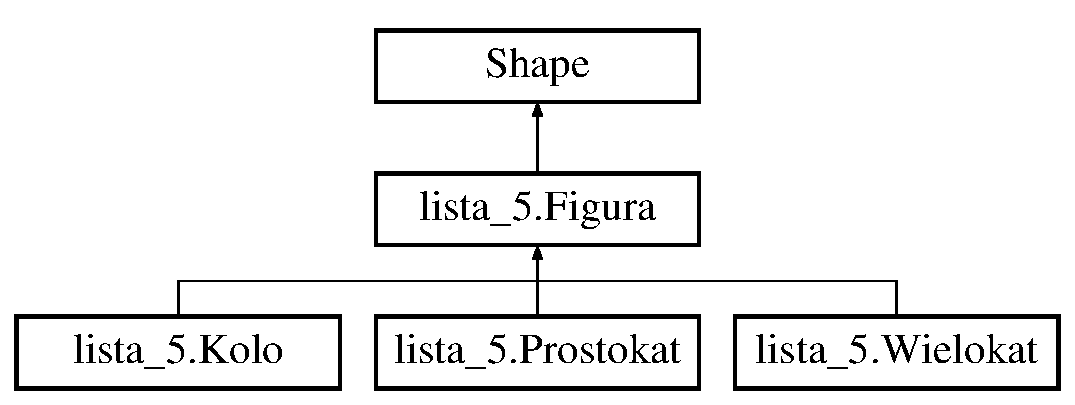
\includegraphics[height=3.000000cm]{interfacelista__5_1_1_figura}
\end{center}
\end{figure}
\subsection*{Public Member Functions}
\begin{DoxyCompactItemize}
\item 
void \mbox{\hyperlink{interfacelista__5_1_1_figura_a1b238957bac675c57febc970067dfd6d}{rysuj}} (Point d)
\item 
void \mbox{\hyperlink{interfacelista__5_1_1_figura_a72f085618cf604e8b1632ea733043861}{przesun}} (int dx, int dy)
\item 
void \mbox{\hyperlink{interfacelista__5_1_1_figura_aaddd90c61fd1632655cb031efafe1a7d}{wypisz\+Dane}} ()
\item 
String \mbox{\hyperlink{interfacelista__5_1_1_figura_a9d60d64b495755a3e48a3eee549a728d}{zapisz\+Dane}} ()
\item 
void \mbox{\hyperlink{interfacelista__5_1_1_figura_a75b72b51014348d839e1f2b81525f264}{ustaw\+Z\+Odczytu}} (String\mbox{[}$\,$\mbox{]} argumenty)
\item 
void \mbox{\hyperlink{interfacelista__5_1_1_figura_aeb0982dc44348dd1fde9266d9d476ed0}{zmien\+Kolor}} (Graphics2D g2d, Color kolor)
\item 
void \mbox{\hyperlink{interfacelista__5_1_1_figura_a3cc13bf7229b288d743be7903b3b61a4}{ustaw\+Kolor}} (Graphics2D g2d)
\item 
void \mbox{\hyperlink{interfacelista__5_1_1_figura_a6813d7ac31e5118bcb34b9b29868ce5f}{zwieksz}} (int zwiekszenie)
\end{DoxyCompactItemize}


\subsection{Detailed Description}
Interfejs kształtów zawierający metody potrzebne każdej rysowanej figurze. Implementują go\+: \mbox{\hyperlink{classlista__5_1_1_kolo}{Kolo}}, \mbox{\hyperlink{classlista__5_1_1_prostokat}{Prostokat}}, \mbox{\hyperlink{classlista__5_1_1_wielokat}{Wielokat}} 

\subsection{Member Function Documentation}
\mbox{\Hypertarget{interfacelista__5_1_1_figura_a72f085618cf604e8b1632ea733043861}\label{interfacelista__5_1_1_figura_a72f085618cf604e8b1632ea733043861}} 
\index{lista\+\_\+5\+::\+Figura@{lista\+\_\+5\+::\+Figura}!przesun@{przesun}}
\index{przesun@{przesun}!lista\+\_\+5\+::\+Figura@{lista\+\_\+5\+::\+Figura}}
\subsubsection{\texorpdfstring{przesun()}{przesun()}}
{\footnotesize\ttfamily void lista\+\_\+5.\+Figura.\+przesun (\begin{DoxyParamCaption}\item[{int}]{dx,  }\item[{int}]{dy }\end{DoxyParamCaption})}

Zmienia położenie figury. 
\begin{DoxyParams}{Parameters}
{\em dx} & zmiana położenia względem osi x, o którą należy przesunąć figurę \\
\hline
{\em dy} & zmiana położenia względem osi y, o którą należy przesunąć figurę \\
\hline
\end{DoxyParams}


Implemented in \mbox{\hyperlink{classlista__5_1_1_kolo_ab984e23d3e45dd5a63dfccf6aeaae01a}{lista\+\_\+5.\+Kolo}}, \mbox{\hyperlink{classlista__5_1_1_prostokat_a9e8a5112287441debbfe24165a24d322}{lista\+\_\+5.\+Prostokat}}, and \mbox{\hyperlink{classlista__5_1_1_wielokat_a565dc0340d5329d74e5f1f7d0eed1049}{lista\+\_\+5.\+Wielokat}}.

\mbox{\Hypertarget{interfacelista__5_1_1_figura_a1b238957bac675c57febc970067dfd6d}\label{interfacelista__5_1_1_figura_a1b238957bac675c57febc970067dfd6d}} 
\index{lista\+\_\+5\+::\+Figura@{lista\+\_\+5\+::\+Figura}!rysuj@{rysuj}}
\index{rysuj@{rysuj}!lista\+\_\+5\+::\+Figura@{lista\+\_\+5\+::\+Figura}}
\subsubsection{\texorpdfstring{rysuj()}{rysuj()}}
{\footnotesize\ttfamily void lista\+\_\+5.\+Figura.\+rysuj (\begin{DoxyParamCaption}\item[{Point}]{d }\end{DoxyParamCaption})}

Zmienia właściwości figury podczas jej tworzenia i rysowania; 
\begin{DoxyParams}{Parameters}
{\em d} & nowy
\begin{DoxyCode}
Point 
\end{DoxyCode}
 , który zmienia kształt figury \\
\hline
\end{DoxyParams}


Implemented in \mbox{\hyperlink{classlista__5_1_1_kolo_acf743c21951288b8794d613665048610}{lista\+\_\+5.\+Kolo}}, \mbox{\hyperlink{classlista__5_1_1_prostokat_a63b2bb7a2b3fd86e21d0d125f4262f39}{lista\+\_\+5.\+Prostokat}}, and \mbox{\hyperlink{classlista__5_1_1_wielokat_aca4b29bcec579f442ac566ec3be96d84}{lista\+\_\+5.\+Wielokat}}.

\mbox{\Hypertarget{interfacelista__5_1_1_figura_a3cc13bf7229b288d743be7903b3b61a4}\label{interfacelista__5_1_1_figura_a3cc13bf7229b288d743be7903b3b61a4}} 
\index{lista\+\_\+5\+::\+Figura@{lista\+\_\+5\+::\+Figura}!ustaw\+Kolor@{ustaw\+Kolor}}
\index{ustaw\+Kolor@{ustaw\+Kolor}!lista\+\_\+5\+::\+Figura@{lista\+\_\+5\+::\+Figura}}
\subsubsection{\texorpdfstring{ustaw\+Kolor()}{ustawKolor()}}
{\footnotesize\ttfamily void lista\+\_\+5.\+Figura.\+ustaw\+Kolor (\begin{DoxyParamCaption}\item[{Graphics2D}]{g2d }\end{DoxyParamCaption})}

Zmienia kolor grafiki na ten, który jest przechowywane w polu kolor. 
\begin{DoxyParams}{Parameters}
{\em g2d} & grafika używana w \mbox{\hyperlink{classlista__5_1_1_wnetrze_aa8676192e150a17230d72de122744a47}{Wnetrze\#paint\+Component}} \\
\hline
\end{DoxyParams}
\begin{DoxySeeAlso}{See also}
\mbox{\hyperlink{interfacelista__5_1_1_figura_aeb0982dc44348dd1fde9266d9d476ed0}{zmien\+Kolor}} 
\end{DoxySeeAlso}


Implemented in \mbox{\hyperlink{classlista__5_1_1_kolo_a97e188acce92c4ca26f1e5483370b00f}{lista\+\_\+5.\+Kolo}}, \mbox{\hyperlink{classlista__5_1_1_prostokat_ad63e4a8c7f291a54f8c9c285c8e6c8ff}{lista\+\_\+5.\+Prostokat}}, and \mbox{\hyperlink{classlista__5_1_1_wielokat_a0c33c8213f6796d16aac592f2a961768}{lista\+\_\+5.\+Wielokat}}.

\mbox{\Hypertarget{interfacelista__5_1_1_figura_a75b72b51014348d839e1f2b81525f264}\label{interfacelista__5_1_1_figura_a75b72b51014348d839e1f2b81525f264}} 
\index{lista\+\_\+5\+::\+Figura@{lista\+\_\+5\+::\+Figura}!ustaw\+Z\+Odczytu@{ustaw\+Z\+Odczytu}}
\index{ustaw\+Z\+Odczytu@{ustaw\+Z\+Odczytu}!lista\+\_\+5\+::\+Figura@{lista\+\_\+5\+::\+Figura}}
\subsubsection{\texorpdfstring{ustaw\+Z\+Odczytu()}{ustawZOdczytu()}}
{\footnotesize\ttfamily void lista\+\_\+5.\+Figura.\+ustaw\+Z\+Odczytu (\begin{DoxyParamCaption}\item[{String \mbox{[}$\,$\mbox{]}}]{argumenty }\end{DoxyParamCaption})}

Ustawia całą figurę korzystając z danych z pliku. 
\begin{DoxyParams}{Parameters}
{\em argumenty} & tablica danych z odczytu, zawiera informacje determinujące figurę \\
\hline
\end{DoxyParams}


Implemented in \mbox{\hyperlink{classlista__5_1_1_wielokat_a8427c86e5be650cbece5464eee1ac053}{lista\+\_\+5.\+Wielokat}}, \mbox{\hyperlink{classlista__5_1_1_prostokat_a93ae9f652ca00886c05be661b17a0886}{lista\+\_\+5.\+Prostokat}}, and \mbox{\hyperlink{classlista__5_1_1_kolo_ad4c6dbc8f29699d8753272098719186e}{lista\+\_\+5.\+Kolo}}.

\mbox{\Hypertarget{interfacelista__5_1_1_figura_aaddd90c61fd1632655cb031efafe1a7d}\label{interfacelista__5_1_1_figura_aaddd90c61fd1632655cb031efafe1a7d}} 
\index{lista\+\_\+5\+::\+Figura@{lista\+\_\+5\+::\+Figura}!wypisz\+Dane@{wypisz\+Dane}}
\index{wypisz\+Dane@{wypisz\+Dane}!lista\+\_\+5\+::\+Figura@{lista\+\_\+5\+::\+Figura}}
\subsubsection{\texorpdfstring{wypisz\+Dane()}{wypiszDane()}}
{\footnotesize\ttfamily void lista\+\_\+5.\+Figura.\+wypisz\+Dane (\begin{DoxyParamCaption}{ }\end{DoxyParamCaption})}

Wypisuje dane związane z figurą w \mbox{\hyperlink{classlista__5_1_1_stopka_a8e8ef21758defd5b137e609b00d2f59e}{Stopka\#dane}} 

Implemented in \mbox{\hyperlink{classlista__5_1_1_kolo_a9b453810cf6823d1f2549f85419aa5a7}{lista\+\_\+5.\+Kolo}}, \mbox{\hyperlink{classlista__5_1_1_prostokat_a95b9ce7b2a7b095c43ffc843cfeff39a}{lista\+\_\+5.\+Prostokat}}, and \mbox{\hyperlink{classlista__5_1_1_wielokat_ad1df79cd3736bb0fcf3ba2252409f3f8}{lista\+\_\+5.\+Wielokat}}.

\mbox{\Hypertarget{interfacelista__5_1_1_figura_a9d60d64b495755a3e48a3eee549a728d}\label{interfacelista__5_1_1_figura_a9d60d64b495755a3e48a3eee549a728d}} 
\index{lista\+\_\+5\+::\+Figura@{lista\+\_\+5\+::\+Figura}!zapisz\+Dane@{zapisz\+Dane}}
\index{zapisz\+Dane@{zapisz\+Dane}!lista\+\_\+5\+::\+Figura@{lista\+\_\+5\+::\+Figura}}
\subsubsection{\texorpdfstring{zapisz\+Dane()}{zapiszDane()}}
{\footnotesize\ttfamily String lista\+\_\+5.\+Figura.\+zapisz\+Dane (\begin{DoxyParamCaption}{ }\end{DoxyParamCaption})}

Przygotowuje informacje o figurze do zapisania. \begin{DoxyReturn}{Returns}
linia, która zostanie zapisana w pliku 
\end{DoxyReturn}


Implemented in \mbox{\hyperlink{classlista__5_1_1_kolo_ab812bc5ce875bf87c7c4268d4f1c8aa2}{lista\+\_\+5.\+Kolo}}, \mbox{\hyperlink{classlista__5_1_1_prostokat_a9537add38b8302420692068fb36726b5}{lista\+\_\+5.\+Prostokat}}, and \mbox{\hyperlink{classlista__5_1_1_wielokat_a6391ebe6bc42d42b6bd3041b1a6bd7bd}{lista\+\_\+5.\+Wielokat}}.

\mbox{\Hypertarget{interfacelista__5_1_1_figura_aeb0982dc44348dd1fde9266d9d476ed0}\label{interfacelista__5_1_1_figura_aeb0982dc44348dd1fde9266d9d476ed0}} 
\index{lista\+\_\+5\+::\+Figura@{lista\+\_\+5\+::\+Figura}!zmien\+Kolor@{zmien\+Kolor}}
\index{zmien\+Kolor@{zmien\+Kolor}!lista\+\_\+5\+::\+Figura@{lista\+\_\+5\+::\+Figura}}
\subsubsection{\texorpdfstring{zmien\+Kolor()}{zmienKolor()}}
{\footnotesize\ttfamily void lista\+\_\+5.\+Figura.\+zmien\+Kolor (\begin{DoxyParamCaption}\item[{Graphics2D}]{g2d,  }\item[{Color}]{kolor }\end{DoxyParamCaption})}

Aktualizuje pole kolor obecne w każdej figurze. 
\begin{DoxyParams}{Parameters}
{\em g2d} & grafika używana w \mbox{\hyperlink{classlista__5_1_1_wnetrze_aa8676192e150a17230d72de122744a47}{Wnetrze\#paint\+Component}} \\
\hline
{\em kolor} & pożądany kolor \\
\hline
\end{DoxyParams}
\begin{DoxySeeAlso}{See also}
\mbox{\hyperlink{interfacelista__5_1_1_figura_a3cc13bf7229b288d743be7903b3b61a4}{ustaw\+Kolor}} 
\end{DoxySeeAlso}


Implemented in \mbox{\hyperlink{classlista__5_1_1_kolo_af4a5e91767dcc103808fb63f39b7404a}{lista\+\_\+5.\+Kolo}}, \mbox{\hyperlink{classlista__5_1_1_prostokat_aa776fbd55cc88f2bb8b8a202109e77ce}{lista\+\_\+5.\+Prostokat}}, and \mbox{\hyperlink{classlista__5_1_1_wielokat_ae863735ff7b742c4703bc142455d34ce}{lista\+\_\+5.\+Wielokat}}.

\mbox{\Hypertarget{interfacelista__5_1_1_figura_a6813d7ac31e5118bcb34b9b29868ce5f}\label{interfacelista__5_1_1_figura_a6813d7ac31e5118bcb34b9b29868ce5f}} 
\index{lista\+\_\+5\+::\+Figura@{lista\+\_\+5\+::\+Figura}!zwieksz@{zwieksz}}
\index{zwieksz@{zwieksz}!lista\+\_\+5\+::\+Figura@{lista\+\_\+5\+::\+Figura}}
\subsubsection{\texorpdfstring{zwieksz()}{zwieksz()}}
{\footnotesize\ttfamily void lista\+\_\+5.\+Figura.\+zwieksz (\begin{DoxyParamCaption}\item[{int}]{zwiekszenie }\end{DoxyParamCaption})}

Powiększa rozmiary figury. 
\begin{DoxyParams}{Parameters}
{\em zwiekszenie} & wartość, o którą należy zwiększyć figurę przy skalowaniu \\
\hline
\end{DoxyParams}


Implemented in \mbox{\hyperlink{classlista__5_1_1_wielokat_a17cfc98331e2a135886070a4094ac0e6}{lista\+\_\+5.\+Wielokat}}, \mbox{\hyperlink{classlista__5_1_1_kolo_a045124cf2c42238baba9ba097c2f5af2}{lista\+\_\+5.\+Kolo}}, and \mbox{\hyperlink{classlista__5_1_1_prostokat_acc961816d5fba86f3442ca34059492f5}{lista\+\_\+5.\+Prostokat}}.



The documentation for this interface was generated from the following file\+:\begin{DoxyCompactItemize}
\item 
lista\+\_\+5/\mbox{\hyperlink{_figura_8java}{Figura.\+java}}\end{DoxyCompactItemize}

\hypertarget{classlista__5_1_1_info}{}\section{lista\+\_\+5.\+Info Class Reference}
\label{classlista__5_1_1_info}\index{lista\+\_\+5.\+Info@{lista\+\_\+5.\+Info}}
Inheritance diagram for lista\+\_\+5.\+Info\+:\begin{figure}[H]
\begin{center}
\leavevmode
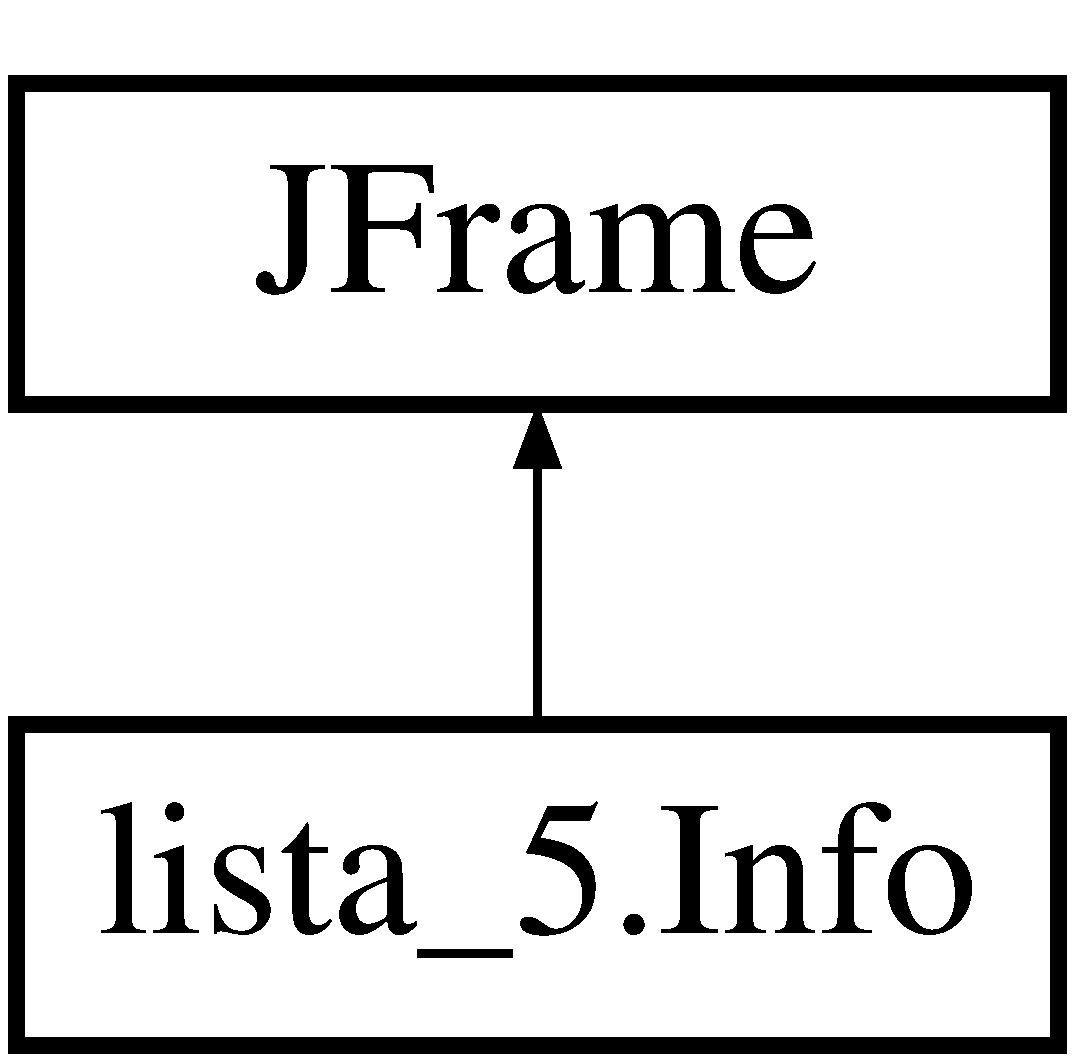
\includegraphics[height=2.000000cm]{classlista__5_1_1_info}
\end{center}
\end{figure}
\subsection*{Public Member Functions}
\begin{DoxyCompactItemize}
\item 
\mbox{\hyperlink{classlista__5_1_1_info_a2485b75de11cae1f2b4a979cb33c875f}{Info}} ()
\end{DoxyCompactItemize}
\subsection*{Private Attributes}
\begin{DoxyCompactItemize}
\item 
J\+Dialog \mbox{\hyperlink{classlista__5_1_1_info_a130163346a8f8eabc00532453d238e4a}{dialog}}
\item 
J\+Text\+Area \mbox{\hyperlink{classlista__5_1_1_info_aef87a771dccda7ab0c438b53904a21e6}{tresc}}
\end{DoxyCompactItemize}


\subsection{Detailed Description}
Klasa zawierająca informacyjne okno dialogowe. 

\subsection{Constructor \& Destructor Documentation}
\mbox{\Hypertarget{classlista__5_1_1_info_a2485b75de11cae1f2b4a979cb33c875f}\label{classlista__5_1_1_info_a2485b75de11cae1f2b4a979cb33c875f}} 
\index{lista\+\_\+5\+::\+Info@{lista\+\_\+5\+::\+Info}!Info@{Info}}
\index{Info@{Info}!lista\+\_\+5\+::\+Info@{lista\+\_\+5\+::\+Info}}
\subsubsection{\texorpdfstring{Info()}{Info()}}
{\footnotesize\ttfamily lista\+\_\+5.\+Info.\+Info (\begin{DoxyParamCaption}{ }\end{DoxyParamCaption})}

Tworzy okno dialogowe i wypełnia je treścią. 

\subsection{Member Data Documentation}
\mbox{\Hypertarget{classlista__5_1_1_info_a130163346a8f8eabc00532453d238e4a}\label{classlista__5_1_1_info_a130163346a8f8eabc00532453d238e4a}} 
\index{lista\+\_\+5\+::\+Info@{lista\+\_\+5\+::\+Info}!dialog@{dialog}}
\index{dialog@{dialog}!lista\+\_\+5\+::\+Info@{lista\+\_\+5\+::\+Info}}
\subsubsection{\texorpdfstring{dialog}{dialog}}
{\footnotesize\ttfamily J\+Dialog lista\+\_\+5.\+Info.\+dialog\hspace{0.3cm}{\ttfamily [private]}}

okno dialogowe z informacjami \mbox{\Hypertarget{classlista__5_1_1_info_aef87a771dccda7ab0c438b53904a21e6}\label{classlista__5_1_1_info_aef87a771dccda7ab0c438b53904a21e6}} 
\index{lista\+\_\+5\+::\+Info@{lista\+\_\+5\+::\+Info}!tresc@{tresc}}
\index{tresc@{tresc}!lista\+\_\+5\+::\+Info@{lista\+\_\+5\+::\+Info}}
\subsubsection{\texorpdfstring{tresc}{tresc}}
{\footnotesize\ttfamily J\+Text\+Area lista\+\_\+5.\+Info.\+tresc\hspace{0.3cm}{\ttfamily [private]}}


\begin{DoxyCode}
JTextArea 
\end{DoxyCode}
 , do której wpisujemy treść informacji 

The documentation for this class was generated from the following file\+:\begin{DoxyCompactItemize}
\item 
lista\+\_\+5/\mbox{\hyperlink{_info_8java}{Info.\+java}}\end{DoxyCompactItemize}

\hypertarget{classlista__5_1_1_kolo}{}\section{lista\+\_\+5.\+Kolo Class Reference}
\label{classlista__5_1_1_kolo}\index{lista\+\_\+5.\+Kolo@{lista\+\_\+5.\+Kolo}}
Inheritance diagram for lista\+\_\+5.\+Kolo\+:\begin{figure}[H]
\begin{center}
\leavevmode
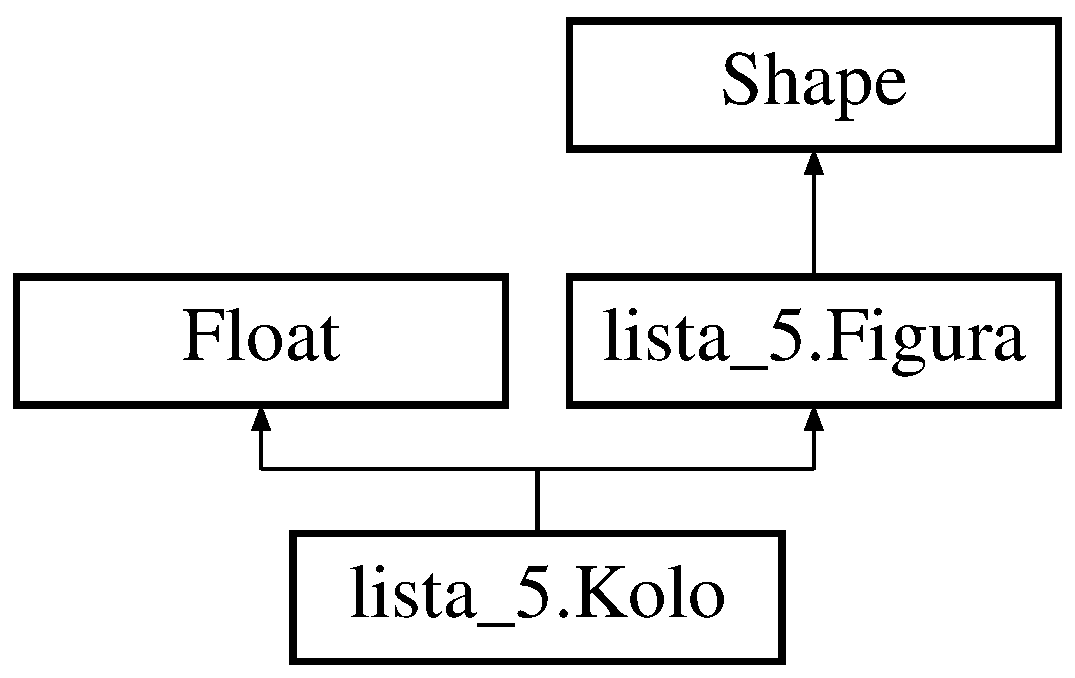
\includegraphics[height=3.000000cm]{classlista__5_1_1_kolo}
\end{center}
\end{figure}
\subsection*{Public Member Functions}
\begin{DoxyCompactItemize}
\item 
\mbox{\hyperlink{classlista__5_1_1_kolo_abbb4dd96b93d0ea773221a321e4af943}{Kolo}} (Point d)
\item 
void \mbox{\hyperlink{classlista__5_1_1_kolo_acf743c21951288b8794d613665048610}{rysuj}} (Point zmienny)
\item 
void \mbox{\hyperlink{classlista__5_1_1_kolo_ab984e23d3e45dd5a63dfccf6aeaae01a}{przesun}} (int dx, int dy)
\item 
void \mbox{\hyperlink{classlista__5_1_1_kolo_a045124cf2c42238baba9ba097c2f5af2}{zwieksz}} (int zwiekszenie)
\item 
void \mbox{\hyperlink{classlista__5_1_1_kolo_ad4c6dbc8f29699d8753272098719186e}{ustaw\+Z\+Odczytu}} (String\mbox{[}$\,$\mbox{]} argumenty)
\item 
void \mbox{\hyperlink{classlista__5_1_1_kolo_a9b453810cf6823d1f2549f85419aa5a7}{wypisz\+Dane}} ()
\item 
String \mbox{\hyperlink{classlista__5_1_1_kolo_ab812bc5ce875bf87c7c4268d4f1c8aa2}{zapisz\+Dane}} ()
\item 
void \mbox{\hyperlink{classlista__5_1_1_kolo_af4a5e91767dcc103808fb63f39b7404a}{zmien\+Kolor}} (Graphics2D g2d, Color \mbox{\hyperlink{classlista__5_1_1_kolo_ae42f8858e1a2278cc04b3190a2ee9fcb}{kolor}})
\item 
void \mbox{\hyperlink{classlista__5_1_1_kolo_a97e188acce92c4ca26f1e5483370b00f}{ustaw\+Kolor}} (Graphics2D g2d)
\end{DoxyCompactItemize}
\subsection*{Private Member Functions}
\begin{DoxyCompactItemize}
\item 
Point \mbox{\hyperlink{classlista__5_1_1_kolo_a4ec5879d3ec849a75bcb1690ed2a0c18}{min}} (Point \mbox{\hyperlink{classlista__5_1_1_kolo_a6deef87b266a0c6c98fc920af90eb81a}{wyjsciowy}}, Point zmienny)
\end{DoxyCompactItemize}
\subsection*{Private Attributes}
\begin{DoxyCompactItemize}
\item 
Point \mbox{\hyperlink{classlista__5_1_1_kolo_a6deef87b266a0c6c98fc920af90eb81a}{wyjsciowy}}
\item 
Color \mbox{\hyperlink{classlista__5_1_1_kolo_ae42f8858e1a2278cc04b3190a2ee9fcb}{kolor}} = Color.\+G\+R\+AY
\item 
final int \mbox{\hyperlink{classlista__5_1_1_kolo_aed784d027c521026966005272339b054}{min\+\_\+width}} = 20
\item 
final int \mbox{\hyperlink{classlista__5_1_1_kolo_a47a917d7de6905904717534ccd188037}{min\+\_\+height}} = 20
\end{DoxyCompactItemize}


\subsection{Detailed Description}
Klasa reprezentująca koło. \begin{DoxySeeAlso}{See also}
\mbox{\hyperlink{interfacelista__5_1_1_figura}{Figura}} 
\end{DoxySeeAlso}


\subsection{Constructor \& Destructor Documentation}
\mbox{\Hypertarget{classlista__5_1_1_kolo_abbb4dd96b93d0ea773221a321e4af943}\label{classlista__5_1_1_kolo_abbb4dd96b93d0ea773221a321e4af943}} 
\index{lista\+\_\+5\+::\+Kolo@{lista\+\_\+5\+::\+Kolo}!Kolo@{Kolo}}
\index{Kolo@{Kolo}!lista\+\_\+5\+::\+Kolo@{lista\+\_\+5\+::\+Kolo}}
\subsubsection{\texorpdfstring{Kolo()}{Kolo()}}
{\footnotesize\ttfamily lista\+\_\+5.\+Kolo.\+Kolo (\begin{DoxyParamCaption}\item[{Point}]{d }\end{DoxyParamCaption})}

Tworzy \mbox{\hyperlink{classlista__5_1_1_kolo}{Kolo}}, ustalając współrzędne punktu wyjsciowego. 
\begin{DoxyParams}{Parameters}
{\em d} & punkt wyjściowy \\
\hline
\end{DoxyParams}
\begin{DoxySeeAlso}{See also}
\mbox{\hyperlink{classlista__5_1_1_kolo_a6deef87b266a0c6c98fc920af90eb81a}{wyjsciowy}} 
\end{DoxySeeAlso}


\subsection{Member Function Documentation}
\mbox{\Hypertarget{classlista__5_1_1_kolo_a4ec5879d3ec849a75bcb1690ed2a0c18}\label{classlista__5_1_1_kolo_a4ec5879d3ec849a75bcb1690ed2a0c18}} 
\index{lista\+\_\+5\+::\+Kolo@{lista\+\_\+5\+::\+Kolo}!min@{min}}
\index{min@{min}!lista\+\_\+5\+::\+Kolo@{lista\+\_\+5\+::\+Kolo}}
\subsubsection{\texorpdfstring{min()}{min()}}
{\footnotesize\ttfamily Point lista\+\_\+5.\+Kolo.\+min (\begin{DoxyParamCaption}\item[{Point}]{wyjsciowy,  }\item[{Point}]{zmienny }\end{DoxyParamCaption})\hspace{0.3cm}{\ttfamily [private]}}

Podaje nam punkt, który powinien być prawym dolnym rogiem tak, aby figura była kołem, a nie elipsą. 
\begin{DoxyParams}{Parameters}
{\em wyjsciowy} & \\
\hline
\end{DoxyParams}
\mbox{\Hypertarget{classlista__5_1_1_kolo_ab984e23d3e45dd5a63dfccf6aeaae01a}\label{classlista__5_1_1_kolo_ab984e23d3e45dd5a63dfccf6aeaae01a}} 
\index{lista\+\_\+5\+::\+Kolo@{lista\+\_\+5\+::\+Kolo}!przesun@{przesun}}
\index{przesun@{przesun}!lista\+\_\+5\+::\+Kolo@{lista\+\_\+5\+::\+Kolo}}
\subsubsection{\texorpdfstring{przesun()}{przesun()}}
{\footnotesize\ttfamily void lista\+\_\+5.\+Kolo.\+przesun (\begin{DoxyParamCaption}\item[{int}]{dx,  }\item[{int}]{dy }\end{DoxyParamCaption})}

Zmienia położenie figury. 
\begin{DoxyParams}{Parameters}
{\em dx} & zmiana położenia względem osi x, o którą należy przesunąć figurę \\
\hline
{\em dy} & zmiana położenia względem osi y, o którą należy przesunąć figurę\\
\hline
\end{DoxyParams}
 

Implements \mbox{\hyperlink{interfacelista__5_1_1_figura_a72f085618cf604e8b1632ea733043861}{lista\+\_\+5.\+Figura}}.

\mbox{\Hypertarget{classlista__5_1_1_kolo_acf743c21951288b8794d613665048610}\label{classlista__5_1_1_kolo_acf743c21951288b8794d613665048610}} 
\index{lista\+\_\+5\+::\+Kolo@{lista\+\_\+5\+::\+Kolo}!rysuj@{rysuj}}
\index{rysuj@{rysuj}!lista\+\_\+5\+::\+Kolo@{lista\+\_\+5\+::\+Kolo}}
\subsubsection{\texorpdfstring{rysuj()}{rysuj()}}
{\footnotesize\ttfamily void lista\+\_\+5.\+Kolo.\+rysuj (\begin{DoxyParamCaption}\item[{Point}]{zmienny }\end{DoxyParamCaption})}

Zmienia właściwości figury podczas jej tworzenia i rysowania; 
\begin{DoxyParams}{Parameters}
{\em d} & nowy
\begin{DoxyCode}
Point 
\end{DoxyCode}
 , który zmienia kształt figury\\
\hline
\end{DoxyParams}
 
\begin{DoxyParams}{Parameters}
{\em zmienny} & prawy dolny róg prostokąta \\
\hline
\end{DoxyParams}


Implements \mbox{\hyperlink{interfacelista__5_1_1_figura_a1b238957bac675c57febc970067dfd6d}{lista\+\_\+5.\+Figura}}.

\mbox{\Hypertarget{classlista__5_1_1_kolo_a97e188acce92c4ca26f1e5483370b00f}\label{classlista__5_1_1_kolo_a97e188acce92c4ca26f1e5483370b00f}} 
\index{lista\+\_\+5\+::\+Kolo@{lista\+\_\+5\+::\+Kolo}!ustaw\+Kolor@{ustaw\+Kolor}}
\index{ustaw\+Kolor@{ustaw\+Kolor}!lista\+\_\+5\+::\+Kolo@{lista\+\_\+5\+::\+Kolo}}
\subsubsection{\texorpdfstring{ustaw\+Kolor()}{ustawKolor()}}
{\footnotesize\ttfamily void lista\+\_\+5.\+Kolo.\+ustaw\+Kolor (\begin{DoxyParamCaption}\item[{Graphics2D}]{g2d }\end{DoxyParamCaption})}

Zmienia kolor grafiki na ten, który jest przechowywane w polu kolor. 
\begin{DoxyParams}{Parameters}
{\em g2d} & grafika używana w \mbox{\hyperlink{classlista__5_1_1_wnetrze_aa8676192e150a17230d72de122744a47}{Wnetrze\#paint\+Component}} \\
\hline
\end{DoxyParams}
\begin{DoxySeeAlso}{See also}
\mbox{\hyperlink{interfacelista__5_1_1_figura_aeb0982dc44348dd1fde9266d9d476ed0}{zmien\+Kolor}}
\end{DoxySeeAlso}
 

Implements \mbox{\hyperlink{interfacelista__5_1_1_figura_a3cc13bf7229b288d743be7903b3b61a4}{lista\+\_\+5.\+Figura}}.

\mbox{\Hypertarget{classlista__5_1_1_kolo_ad4c6dbc8f29699d8753272098719186e}\label{classlista__5_1_1_kolo_ad4c6dbc8f29699d8753272098719186e}} 
\index{lista\+\_\+5\+::\+Kolo@{lista\+\_\+5\+::\+Kolo}!ustaw\+Z\+Odczytu@{ustaw\+Z\+Odczytu}}
\index{ustaw\+Z\+Odczytu@{ustaw\+Z\+Odczytu}!lista\+\_\+5\+::\+Kolo@{lista\+\_\+5\+::\+Kolo}}
\subsubsection{\texorpdfstring{ustaw\+Z\+Odczytu()}{ustawZOdczytu()}}
{\footnotesize\ttfamily void lista\+\_\+5.\+Kolo.\+ustaw\+Z\+Odczytu (\begin{DoxyParamCaption}\item[{String \mbox{[}$\,$\mbox{]}}]{argumenty }\end{DoxyParamCaption})}

Ustawia całą figurę korzystając z danych z pliku. 
\begin{DoxyParams}{Parameters}
{\em argumenty} & tablica danych z odczytu, zawiera informacje determinujące figurę\\
\hline
\end{DoxyParams}
 

Implements \mbox{\hyperlink{interfacelista__5_1_1_figura_a75b72b51014348d839e1f2b81525f264}{lista\+\_\+5.\+Figura}}.

\mbox{\Hypertarget{classlista__5_1_1_kolo_a9b453810cf6823d1f2549f85419aa5a7}\label{classlista__5_1_1_kolo_a9b453810cf6823d1f2549f85419aa5a7}} 
\index{lista\+\_\+5\+::\+Kolo@{lista\+\_\+5\+::\+Kolo}!wypisz\+Dane@{wypisz\+Dane}}
\index{wypisz\+Dane@{wypisz\+Dane}!lista\+\_\+5\+::\+Kolo@{lista\+\_\+5\+::\+Kolo}}
\subsubsection{\texorpdfstring{wypisz\+Dane()}{wypiszDane()}}
{\footnotesize\ttfamily void lista\+\_\+5.\+Kolo.\+wypisz\+Dane (\begin{DoxyParamCaption}{ }\end{DoxyParamCaption})}

Wypisuje dane związane z figurą w \mbox{\hyperlink{classlista__5_1_1_stopka_a8e8ef21758defd5b137e609b00d2f59e}{Stopka\#dane}} 

Implements \mbox{\hyperlink{interfacelista__5_1_1_figura_aaddd90c61fd1632655cb031efafe1a7d}{lista\+\_\+5.\+Figura}}.

\mbox{\Hypertarget{classlista__5_1_1_kolo_ab812bc5ce875bf87c7c4268d4f1c8aa2}\label{classlista__5_1_1_kolo_ab812bc5ce875bf87c7c4268d4f1c8aa2}} 
\index{lista\+\_\+5\+::\+Kolo@{lista\+\_\+5\+::\+Kolo}!zapisz\+Dane@{zapisz\+Dane}}
\index{zapisz\+Dane@{zapisz\+Dane}!lista\+\_\+5\+::\+Kolo@{lista\+\_\+5\+::\+Kolo}}
\subsubsection{\texorpdfstring{zapisz\+Dane()}{zapiszDane()}}
{\footnotesize\ttfamily String lista\+\_\+5.\+Kolo.\+zapisz\+Dane (\begin{DoxyParamCaption}{ }\end{DoxyParamCaption})}

Przygotowuje informacje o figurze do zapisania. \begin{DoxyReturn}{Returns}
linia, która zostanie zapisana w pliku
\end{DoxyReturn}
 

Implements \mbox{\hyperlink{interfacelista__5_1_1_figura_a9d60d64b495755a3e48a3eee549a728d}{lista\+\_\+5.\+Figura}}.

\mbox{\Hypertarget{classlista__5_1_1_kolo_af4a5e91767dcc103808fb63f39b7404a}\label{classlista__5_1_1_kolo_af4a5e91767dcc103808fb63f39b7404a}} 
\index{lista\+\_\+5\+::\+Kolo@{lista\+\_\+5\+::\+Kolo}!zmien\+Kolor@{zmien\+Kolor}}
\index{zmien\+Kolor@{zmien\+Kolor}!lista\+\_\+5\+::\+Kolo@{lista\+\_\+5\+::\+Kolo}}
\subsubsection{\texorpdfstring{zmien\+Kolor()}{zmienKolor()}}
{\footnotesize\ttfamily void lista\+\_\+5.\+Kolo.\+zmien\+Kolor (\begin{DoxyParamCaption}\item[{Graphics2D}]{g2d,  }\item[{Color}]{kolor }\end{DoxyParamCaption})}

Aktualizuje pole kolor obecne w każdej figurze. 
\begin{DoxyParams}{Parameters}
{\em g2d} & grafika używana w \mbox{\hyperlink{classlista__5_1_1_wnetrze_aa8676192e150a17230d72de122744a47}{Wnetrze\#paint\+Component}} \\
\hline
{\em kolor} & pożądany kolor \\
\hline
\end{DoxyParams}
\begin{DoxySeeAlso}{See also}
\mbox{\hyperlink{interfacelista__5_1_1_figura_a3cc13bf7229b288d743be7903b3b61a4}{ustaw\+Kolor}}
\end{DoxySeeAlso}
 

Implements \mbox{\hyperlink{interfacelista__5_1_1_figura_aeb0982dc44348dd1fde9266d9d476ed0}{lista\+\_\+5.\+Figura}}.

\mbox{\Hypertarget{classlista__5_1_1_kolo_a045124cf2c42238baba9ba097c2f5af2}\label{classlista__5_1_1_kolo_a045124cf2c42238baba9ba097c2f5af2}} 
\index{lista\+\_\+5\+::\+Kolo@{lista\+\_\+5\+::\+Kolo}!zwieksz@{zwieksz}}
\index{zwieksz@{zwieksz}!lista\+\_\+5\+::\+Kolo@{lista\+\_\+5\+::\+Kolo}}
\subsubsection{\texorpdfstring{zwieksz()}{zwieksz()}}
{\footnotesize\ttfamily void lista\+\_\+5.\+Kolo.\+zwieksz (\begin{DoxyParamCaption}\item[{int}]{zwiekszenie }\end{DoxyParamCaption})}

Powiększa rozmiary figury. 
\begin{DoxyParams}{Parameters}
{\em zwiekszenie} & wartość, o którą należy zwiększyć figurę przy skalowaniu\\
\hline
\end{DoxyParams}
, pamiętając o wartościach minimalnych. \begin{DoxySeeAlso}{See also}
\mbox{\hyperlink{classlista__5_1_1_kolo_aed784d027c521026966005272339b054}{min\+\_\+width}} 

\mbox{\hyperlink{classlista__5_1_1_kolo_a47a917d7de6905904717534ccd188037}{min\+\_\+height}} 
\end{DoxySeeAlso}


Implements \mbox{\hyperlink{interfacelista__5_1_1_figura_a6813d7ac31e5118bcb34b9b29868ce5f}{lista\+\_\+5.\+Figura}}.



\subsection{Member Data Documentation}
\mbox{\Hypertarget{classlista__5_1_1_kolo_ae42f8858e1a2278cc04b3190a2ee9fcb}\label{classlista__5_1_1_kolo_ae42f8858e1a2278cc04b3190a2ee9fcb}} 
\index{lista\+\_\+5\+::\+Kolo@{lista\+\_\+5\+::\+Kolo}!kolor@{kolor}}
\index{kolor@{kolor}!lista\+\_\+5\+::\+Kolo@{lista\+\_\+5\+::\+Kolo}}
\subsubsection{\texorpdfstring{kolor}{kolor}}
{\footnotesize\ttfamily Color lista\+\_\+5.\+Kolo.\+kolor = Color.\+G\+R\+AY\hspace{0.3cm}{\ttfamily [private]}}


\begin{DoxyCode}
Color 
\end{DoxyCode}
 , domyślnie ustawiony na
\begin{DoxyCode}
Color.GRAY 
\end{DoxyCode}
 \mbox{\Hypertarget{classlista__5_1_1_kolo_a47a917d7de6905904717534ccd188037}\label{classlista__5_1_1_kolo_a47a917d7de6905904717534ccd188037}} 
\index{lista\+\_\+5\+::\+Kolo@{lista\+\_\+5\+::\+Kolo}!min\+\_\+height@{min\+\_\+height}}
\index{min\+\_\+height@{min\+\_\+height}!lista\+\_\+5\+::\+Kolo@{lista\+\_\+5\+::\+Kolo}}
\subsubsection{\texorpdfstring{min\+\_\+height}{min\_height}}
{\footnotesize\ttfamily final int lista\+\_\+5.\+Kolo.\+min\+\_\+height = 20\hspace{0.3cm}{\ttfamily [private]}}

Minimalna wysokość, która jest nieprzekraczalna przy zmniejszaniu. \mbox{\Hypertarget{classlista__5_1_1_kolo_aed784d027c521026966005272339b054}\label{classlista__5_1_1_kolo_aed784d027c521026966005272339b054}} 
\index{lista\+\_\+5\+::\+Kolo@{lista\+\_\+5\+::\+Kolo}!min\+\_\+width@{min\+\_\+width}}
\index{min\+\_\+width@{min\+\_\+width}!lista\+\_\+5\+::\+Kolo@{lista\+\_\+5\+::\+Kolo}}
\subsubsection{\texorpdfstring{min\+\_\+width}{min\_width}}
{\footnotesize\ttfamily final int lista\+\_\+5.\+Kolo.\+min\+\_\+width = 20\hspace{0.3cm}{\ttfamily [private]}}

Minimalna szerokość, która jest nieprzekraczalna przy zmniejszaniu. \mbox{\Hypertarget{classlista__5_1_1_kolo_a6deef87b266a0c6c98fc920af90eb81a}\label{classlista__5_1_1_kolo_a6deef87b266a0c6c98fc920af90eb81a}} 
\index{lista\+\_\+5\+::\+Kolo@{lista\+\_\+5\+::\+Kolo}!wyjsciowy@{wyjsciowy}}
\index{wyjsciowy@{wyjsciowy}!lista\+\_\+5\+::\+Kolo@{lista\+\_\+5\+::\+Kolo}}
\subsubsection{\texorpdfstring{wyjsciowy}{wyjsciowy}}
{\footnotesize\ttfamily Point lista\+\_\+5.\+Kolo.\+wyjsciowy\hspace{0.3cm}{\ttfamily [private]}}

wyjsciowy
\begin{DoxyCode}
Point 
\end{DoxyCode}
 , lewy górny róg okalającego prostokąta, niezmienny przy rysowaniu 

The documentation for this class was generated from the following file\+:\begin{DoxyCompactItemize}
\item 
lista\+\_\+5/\mbox{\hyperlink{_kolo_8java}{Kolo.\+java}}\end{DoxyCompactItemize}

\hypertarget{classlista__5_1_1_menu_kontekstowe}{}\section{lista\+\_\+5.\+Menu\+Kontekstowe Class Reference}
\label{classlista__5_1_1_menu_kontekstowe}\index{lista\+\_\+5.\+Menu\+Kontekstowe@{lista\+\_\+5.\+Menu\+Kontekstowe}}
Inheritance diagram for lista\+\_\+5.\+Menu\+Kontekstowe\+:\begin{figure}[H]
\begin{center}
\leavevmode
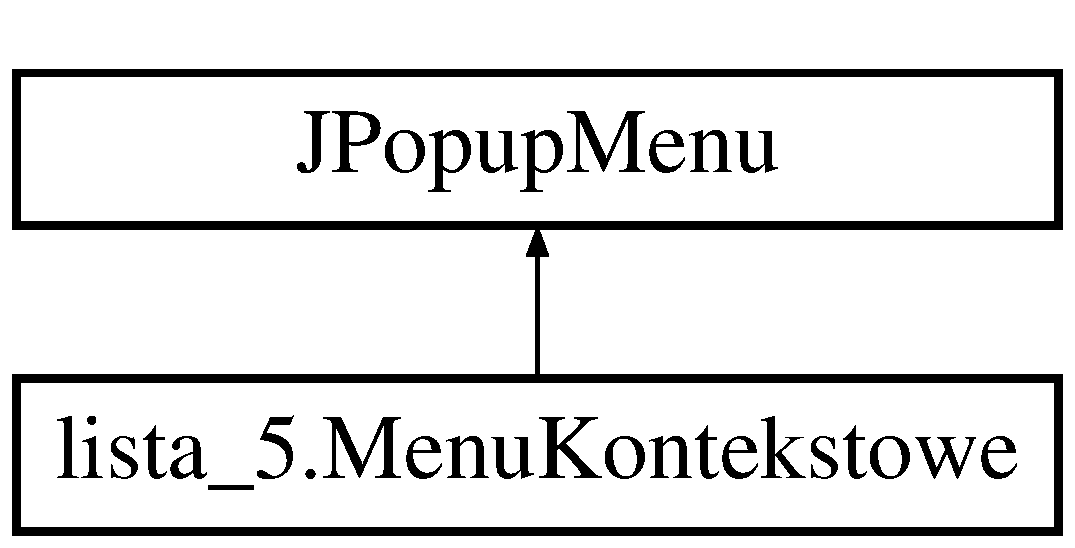
\includegraphics[height=2.000000cm]{classlista__5_1_1_menu_kontekstowe}
\end{center}
\end{figure}
\subsection*{Public Member Functions}
\begin{DoxyCompactItemize}
\item 
\mbox{\hyperlink{classlista__5_1_1_menu_kontekstowe_a1ea2acb59485840515086be771eb0d5f}{Menu\+Kontekstowe}} ()
\end{DoxyCompactItemize}
\subsection*{Public Attributes}
\begin{DoxyCompactItemize}
\item 
Color \mbox{[}$\,$\mbox{]} \mbox{\hyperlink{classlista__5_1_1_menu_kontekstowe_ae96bde96586b2e16da0b5d18bc679f4c}{kolory}} = \{ Color.\+R\+ED, Color.\+G\+R\+E\+EN, Color.\+Y\+E\+L\+L\+OW, Color.\+M\+A\+G\+E\+N\+TA, new Color(210, 246, 255) \}
\item 
J\+Menu\+Item \mbox{[}$\,$\mbox{]} \mbox{\hyperlink{classlista__5_1_1_menu_kontekstowe_a95c06de0ee36c780699c2a1efa4b30d0}{wypelnienia}}
\end{DoxyCompactItemize}
\subsection*{Private Member Functions}
\begin{DoxyCompactItemize}
\item 
void \mbox{\hyperlink{classlista__5_1_1_menu_kontekstowe_a374ed94eba427019665e64c496c6bc9b}{ustaw\+Wypelnienia}} ()
\end{DoxyCompactItemize}


\subsection{Detailed Description}
Implementacja menu kontekstowego służącego do zmiany koloru figury. 

\subsection{Constructor \& Destructor Documentation}
\mbox{\Hypertarget{classlista__5_1_1_menu_kontekstowe_a1ea2acb59485840515086be771eb0d5f}\label{classlista__5_1_1_menu_kontekstowe_a1ea2acb59485840515086be771eb0d5f}} 
\index{lista\+\_\+5\+::\+Menu\+Kontekstowe@{lista\+\_\+5\+::\+Menu\+Kontekstowe}!Menu\+Kontekstowe@{Menu\+Kontekstowe}}
\index{Menu\+Kontekstowe@{Menu\+Kontekstowe}!lista\+\_\+5\+::\+Menu\+Kontekstowe@{lista\+\_\+5\+::\+Menu\+Kontekstowe}}
\subsubsection{\texorpdfstring{Menu\+Kontekstowe()}{MenuKontekstowe()}}
{\footnotesize\ttfamily lista\+\_\+5.\+Menu\+Kontekstowe.\+Menu\+Kontekstowe (\begin{DoxyParamCaption}{ }\end{DoxyParamCaption})}

Tworzy menu. 

\subsection{Member Function Documentation}
\mbox{\Hypertarget{classlista__5_1_1_menu_kontekstowe_a374ed94eba427019665e64c496c6bc9b}\label{classlista__5_1_1_menu_kontekstowe_a374ed94eba427019665e64c496c6bc9b}} 
\index{lista\+\_\+5\+::\+Menu\+Kontekstowe@{lista\+\_\+5\+::\+Menu\+Kontekstowe}!ustaw\+Wypelnienia@{ustaw\+Wypelnienia}}
\index{ustaw\+Wypelnienia@{ustaw\+Wypelnienia}!lista\+\_\+5\+::\+Menu\+Kontekstowe@{lista\+\_\+5\+::\+Menu\+Kontekstowe}}
\subsubsection{\texorpdfstring{ustaw\+Wypelnienia()}{ustawWypelnienia()}}
{\footnotesize\ttfamily void lista\+\_\+5.\+Menu\+Kontekstowe.\+ustaw\+Wypelnienia (\begin{DoxyParamCaption}{ }\end{DoxyParamCaption})\hspace{0.3cm}{\ttfamily [private]}}

tworzy J\+Menu\+Item, koloruje, ustawia wielkość i dodaje je (indeksy z wypelnienia\mbox{[}\mbox{]} odpowiadają kolory\mbox{[}\mbox{]} od 0 do 4) 

\subsection{Member Data Documentation}
\mbox{\Hypertarget{classlista__5_1_1_menu_kontekstowe_ae96bde96586b2e16da0b5d18bc679f4c}\label{classlista__5_1_1_menu_kontekstowe_ae96bde96586b2e16da0b5d18bc679f4c}} 
\index{lista\+\_\+5\+::\+Menu\+Kontekstowe@{lista\+\_\+5\+::\+Menu\+Kontekstowe}!kolory@{kolory}}
\index{kolory@{kolory}!lista\+\_\+5\+::\+Menu\+Kontekstowe@{lista\+\_\+5\+::\+Menu\+Kontekstowe}}
\subsubsection{\texorpdfstring{kolory}{kolory}}
{\footnotesize\ttfamily Color \mbox{[}$\,$\mbox{]} lista\+\_\+5.\+Menu\+Kontekstowe.\+kolory = \{ Color.\+R\+ED, Color.\+G\+R\+E\+EN, Color.\+Y\+E\+L\+L\+OW, Color.\+M\+A\+G\+E\+N\+TA, new Color(210, 246, 255) \}}

tablica przechowująca możliwe do wybrania kolory \mbox{\Hypertarget{classlista__5_1_1_menu_kontekstowe_a95c06de0ee36c780699c2a1efa4b30d0}\label{classlista__5_1_1_menu_kontekstowe_a95c06de0ee36c780699c2a1efa4b30d0}} 
\index{lista\+\_\+5\+::\+Menu\+Kontekstowe@{lista\+\_\+5\+::\+Menu\+Kontekstowe}!wypelnienia@{wypelnienia}}
\index{wypelnienia@{wypelnienia}!lista\+\_\+5\+::\+Menu\+Kontekstowe@{lista\+\_\+5\+::\+Menu\+Kontekstowe}}
\subsubsection{\texorpdfstring{wypelnienia}{wypelnienia}}
{\footnotesize\ttfamily J\+Menu\+Item \mbox{[}$\,$\mbox{]} lista\+\_\+5.\+Menu\+Kontekstowe.\+wypelnienia}

tablica przechowująca przyciski służące do zmiany koloru 

The documentation for this class was generated from the following file\+:\begin{DoxyCompactItemize}
\item 
lista\+\_\+5/\mbox{\hyperlink{_menu_kontekstowe_8java}{Menu\+Kontekstowe.\+java}}\end{DoxyCompactItemize}

\hypertarget{classlista__5_1_1_wnetrze_1_1_moj_mouse_adapter}{}\section{lista\+\_\+5.\+Wnetrze.\+Moj\+Mouse\+Adapter Class Reference}
\label{classlista__5_1_1_wnetrze_1_1_moj_mouse_adapter}\index{lista\+\_\+5.\+Wnetrze.\+Moj\+Mouse\+Adapter@{lista\+\_\+5.\+Wnetrze.\+Moj\+Mouse\+Adapter}}
Inheritance diagram for lista\+\_\+5.\+Wnetrze.\+Moj\+Mouse\+Adapter\+:\begin{figure}[H]
\begin{center}
\leavevmode
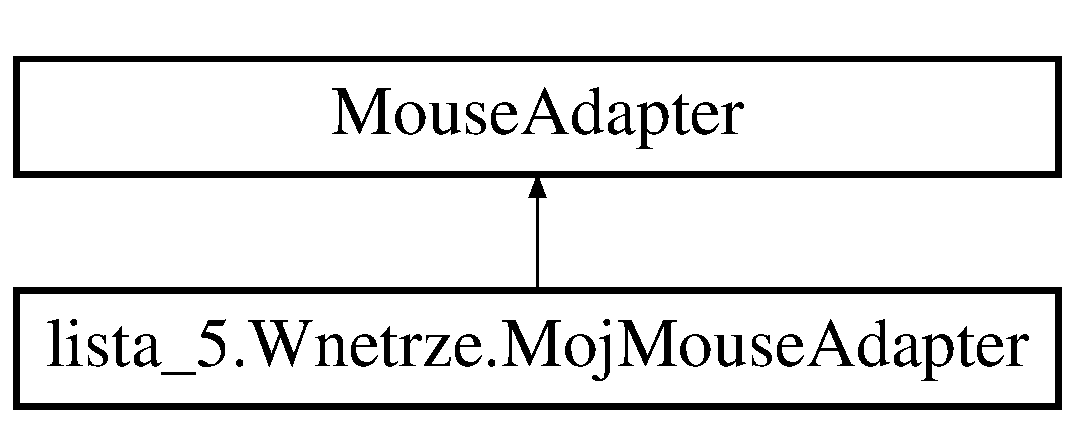
\includegraphics[height=2.000000cm]{classlista__5_1_1_wnetrze_1_1_moj_mouse_adapter}
\end{center}
\end{figure}
\subsection*{Public Member Functions}
\begin{DoxyCompactItemize}
\item 
void \mbox{\hyperlink{classlista__5_1_1_wnetrze_1_1_moj_mouse_adapter_a4ef4404b4f86ad51e68805d24d8c77b2}{mouse\+Pressed}} (Mouse\+Event e)
\item 
void \mbox{\hyperlink{classlista__5_1_1_wnetrze_1_1_moj_mouse_adapter_a37c0d26aa18789ec52ba5acc80251de4}{mouse\+Dragged}} (Mouse\+Event e)
\item 
void \mbox{\hyperlink{classlista__5_1_1_wnetrze_1_1_moj_mouse_adapter_a1835ceb6a8d4d0519e1473ae586f73cc}{mouse\+Clicked}} (Mouse\+Event e)
\item 
void \mbox{\hyperlink{classlista__5_1_1_wnetrze_1_1_moj_mouse_adapter_a782d984136df2ccfa45c7968931b6eff}{mouse\+Released}} (Mouse\+Event e)
\item 
void \mbox{\hyperlink{classlista__5_1_1_wnetrze_1_1_moj_mouse_adapter_a49b07d26c2eb16d94ec11104f9d60779}{mouse\+Wheel\+Moved}} (Mouse\+Wheel\+Event e)
\end{DoxyCompactItemize}
\subsection*{Private Member Functions}
\begin{DoxyCompactItemize}
\item 
void \mbox{\hyperlink{classlista__5_1_1_wnetrze_1_1_moj_mouse_adapter_acaa74559dde8d1028b6cee91e91d5d20}{tworz\+Menu}} (Mouse\+Event e)
\end{DoxyCompactItemize}
\subsection*{Private Attributes}
\begin{DoxyCompactItemize}
\item 
\mbox{\hyperlink{interfacelista__5_1_1_figura}{Figura}} \mbox{\hyperlink{classlista__5_1_1_wnetrze_1_1_moj_mouse_adapter_a21bbd36a0f45068c966e26c532b2421c}{figura\+Rys}}
\item 
\mbox{\hyperlink{interfacelista__5_1_1_figura}{Figura}} \mbox{\hyperlink{classlista__5_1_1_wnetrze_1_1_moj_mouse_adapter_a99de9fbdf459dc4783c71017a73cae3a}{figura\+Przes}}
\item 
Point \mbox{\hyperlink{classlista__5_1_1_wnetrze_1_1_moj_mouse_adapter_a54478d4d410971228cd0821c48645193}{przesuwanie}}
\item 
boolean \mbox{\hyperlink{classlista__5_1_1_wnetrze_1_1_moj_mouse_adapter_a2ddea923bcec57d12727dbc5bf7c2e05}{czy\+Wewnatrz}} = false
\end{DoxyCompactItemize}


\subsection{Detailed Description}
Obsługuje wszystkie zdarzenia związane z myszką. 

\subsection{Member Function Documentation}
\mbox{\Hypertarget{classlista__5_1_1_wnetrze_1_1_moj_mouse_adapter_a1835ceb6a8d4d0519e1473ae586f73cc}\label{classlista__5_1_1_wnetrze_1_1_moj_mouse_adapter_a1835ceb6a8d4d0519e1473ae586f73cc}} 
\index{lista\+\_\+5\+::\+Wnetrze\+::\+Moj\+Mouse\+Adapter@{lista\+\_\+5\+::\+Wnetrze\+::\+Moj\+Mouse\+Adapter}!mouse\+Clicked@{mouse\+Clicked}}
\index{mouse\+Clicked@{mouse\+Clicked}!lista\+\_\+5\+::\+Wnetrze\+::\+Moj\+Mouse\+Adapter@{lista\+\_\+5\+::\+Wnetrze\+::\+Moj\+Mouse\+Adapter}}
\subsubsection{\texorpdfstring{mouse\+Clicked()}{mouseClicked()}}
{\footnotesize\ttfamily void lista\+\_\+5.\+Wnetrze.\+Moj\+Mouse\+Adapter.\+mouse\+Clicked (\begin{DoxyParamCaption}\item[{Mouse\+Event}]{e }\end{DoxyParamCaption})}

W trybie tworzenia tworzy wielokąt. W trybie edycji uruchamia metodę służącą do tworzenia menu. Najpierw wywołuje się \mbox{\hyperlink{classlista__5_1_1_wnetrze_1_1_moj_mouse_adapter_a782d984136df2ccfa45c7968931b6eff}{mouse\+Released}}, następnie
\begin{DoxyCode}
\mbox{\hyperlink{classlista__5_1_1_wnetrze_1_1_moj_mouse_adapter_a1835ceb6a8d4d0519e1473ae586f73cc}{mouseClicked}} 
\end{DoxyCode}
 . 
\begin{DoxyParams}{Parameters}
{\em e} & zdarzenie związane z kliknięciem przycisku myszy \\
\hline
\end{DoxyParams}
\mbox{\Hypertarget{classlista__5_1_1_wnetrze_1_1_moj_mouse_adapter_a37c0d26aa18789ec52ba5acc80251de4}\label{classlista__5_1_1_wnetrze_1_1_moj_mouse_adapter_a37c0d26aa18789ec52ba5acc80251de4}} 
\index{lista\+\_\+5\+::\+Wnetrze\+::\+Moj\+Mouse\+Adapter@{lista\+\_\+5\+::\+Wnetrze\+::\+Moj\+Mouse\+Adapter}!mouse\+Dragged@{mouse\+Dragged}}
\index{mouse\+Dragged@{mouse\+Dragged}!lista\+\_\+5\+::\+Wnetrze\+::\+Moj\+Mouse\+Adapter@{lista\+\_\+5\+::\+Wnetrze\+::\+Moj\+Mouse\+Adapter}}
\subsubsection{\texorpdfstring{mouse\+Dragged()}{mouseDragged()}}
{\footnotesize\ttfamily void lista\+\_\+5.\+Wnetrze.\+Moj\+Mouse\+Adapter.\+mouse\+Dragged (\begin{DoxyParamCaption}\item[{Mouse\+Event}]{e }\end{DoxyParamCaption})}

W trybie tworzenia pozwala rozszerzać figurę, w trybie edycji przesuwa ją i uruchamia wypisywanie danych w \mbox{\hyperlink{classlista__5_1_1_stopka_a8e8ef21758defd5b137e609b00d2f59e}{Stopka\#dane}}. 
\begin{DoxyParams}{Parameters}
{\em e} & zdarzenie związane z przesunięciem myszy \\
\hline
\end{DoxyParams}
\mbox{\Hypertarget{classlista__5_1_1_wnetrze_1_1_moj_mouse_adapter_a4ef4404b4f86ad51e68805d24d8c77b2}\label{classlista__5_1_1_wnetrze_1_1_moj_mouse_adapter_a4ef4404b4f86ad51e68805d24d8c77b2}} 
\index{lista\+\_\+5\+::\+Wnetrze\+::\+Moj\+Mouse\+Adapter@{lista\+\_\+5\+::\+Wnetrze\+::\+Moj\+Mouse\+Adapter}!mouse\+Pressed@{mouse\+Pressed}}
\index{mouse\+Pressed@{mouse\+Pressed}!lista\+\_\+5\+::\+Wnetrze\+::\+Moj\+Mouse\+Adapter@{lista\+\_\+5\+::\+Wnetrze\+::\+Moj\+Mouse\+Adapter}}
\subsubsection{\texorpdfstring{mouse\+Pressed()}{mousePressed()}}
{\footnotesize\ttfamily void lista\+\_\+5.\+Wnetrze.\+Moj\+Mouse\+Adapter.\+mouse\+Pressed (\begin{DoxyParamCaption}\item[{Mouse\+Event}]{e }\end{DoxyParamCaption})}

W trybie tworzenia tworzy koła i prostokąty, w trybie edycji przygotowuje przesuwanie. 
\begin{DoxyParams}{Parameters}
{\em e} & zdarzenie związane z wciśnięciem myszy \\
\hline
\end{DoxyParams}
\mbox{\Hypertarget{classlista__5_1_1_wnetrze_1_1_moj_mouse_adapter_a782d984136df2ccfa45c7968931b6eff}\label{classlista__5_1_1_wnetrze_1_1_moj_mouse_adapter_a782d984136df2ccfa45c7968931b6eff}} 
\index{lista\+\_\+5\+::\+Wnetrze\+::\+Moj\+Mouse\+Adapter@{lista\+\_\+5\+::\+Wnetrze\+::\+Moj\+Mouse\+Adapter}!mouse\+Released@{mouse\+Released}}
\index{mouse\+Released@{mouse\+Released}!lista\+\_\+5\+::\+Wnetrze\+::\+Moj\+Mouse\+Adapter@{lista\+\_\+5\+::\+Wnetrze\+::\+Moj\+Mouse\+Adapter}}
\subsubsection{\texorpdfstring{mouse\+Released()}{mouseReleased()}}
{\footnotesize\ttfamily void lista\+\_\+5.\+Wnetrze.\+Moj\+Mouse\+Adapter.\+mouse\+Released (\begin{DoxyParamCaption}\item[{Mouse\+Event}]{e }\end{DoxyParamCaption})}

W trybie tworzenia sprawia, że przyciski się odklikują lub blokują, by nie doszło do konfliktów. W trybie edycji tworzy menu. 
\begin{DoxyParams}{Parameters}
{\em e} & zdarzenie związane ze zwolnieniem przycisku myszy \\
\hline
\end{DoxyParams}
\mbox{\Hypertarget{classlista__5_1_1_wnetrze_1_1_moj_mouse_adapter_a49b07d26c2eb16d94ec11104f9d60779}\label{classlista__5_1_1_wnetrze_1_1_moj_mouse_adapter_a49b07d26c2eb16d94ec11104f9d60779}} 
\index{lista\+\_\+5\+::\+Wnetrze\+::\+Moj\+Mouse\+Adapter@{lista\+\_\+5\+::\+Wnetrze\+::\+Moj\+Mouse\+Adapter}!mouse\+Wheel\+Moved@{mouse\+Wheel\+Moved}}
\index{mouse\+Wheel\+Moved@{mouse\+Wheel\+Moved}!lista\+\_\+5\+::\+Wnetrze\+::\+Moj\+Mouse\+Adapter@{lista\+\_\+5\+::\+Wnetrze\+::\+Moj\+Mouse\+Adapter}}
\subsubsection{\texorpdfstring{mouse\+Wheel\+Moved()}{mouseWheelMoved()}}
{\footnotesize\ttfamily void lista\+\_\+5.\+Wnetrze.\+Moj\+Mouse\+Adapter.\+mouse\+Wheel\+Moved (\begin{DoxyParamCaption}\item[{Mouse\+Wheel\+Event}]{e }\end{DoxyParamCaption})}

Dla każdej figury, która zawiera punkt, w którym obecnie znajduje się przycisk myszy, wywołuje metodę \mbox{\hyperlink{interfacelista__5_1_1_figura_a6813d7ac31e5118bcb34b9b29868ce5f}{Figura\#zwieksz(int)}} 
\begin{DoxyParams}{Parameters}
{\em e} & zdarzenie związane z poruszeniem scrolla \\
\hline
\end{DoxyParams}
\mbox{\Hypertarget{classlista__5_1_1_wnetrze_1_1_moj_mouse_adapter_acaa74559dde8d1028b6cee91e91d5d20}\label{classlista__5_1_1_wnetrze_1_1_moj_mouse_adapter_acaa74559dde8d1028b6cee91e91d5d20}} 
\index{lista\+\_\+5\+::\+Wnetrze\+::\+Moj\+Mouse\+Adapter@{lista\+\_\+5\+::\+Wnetrze\+::\+Moj\+Mouse\+Adapter}!tworz\+Menu@{tworz\+Menu}}
\index{tworz\+Menu@{tworz\+Menu}!lista\+\_\+5\+::\+Wnetrze\+::\+Moj\+Mouse\+Adapter@{lista\+\_\+5\+::\+Wnetrze\+::\+Moj\+Mouse\+Adapter}}
\subsubsection{\texorpdfstring{tworz\+Menu()}{tworzMenu()}}
{\footnotesize\ttfamily void lista\+\_\+5.\+Wnetrze.\+Moj\+Mouse\+Adapter.\+tworz\+Menu (\begin{DoxyParamCaption}\item[{Mouse\+Event}]{e }\end{DoxyParamCaption})\hspace{0.3cm}{\ttfamily [private]}}

Sprawdza, czy należy stworzyć menu, jeśli tak -\/ robi to. 
\begin{DoxyParams}{Parameters}
{\em e} & zdarzenie związane z kliknięciem na terenie panelu \\
\hline
\end{DoxyParams}


\subsection{Member Data Documentation}
\mbox{\Hypertarget{classlista__5_1_1_wnetrze_1_1_moj_mouse_adapter_a2ddea923bcec57d12727dbc5bf7c2e05}\label{classlista__5_1_1_wnetrze_1_1_moj_mouse_adapter_a2ddea923bcec57d12727dbc5bf7c2e05}} 
\index{lista\+\_\+5\+::\+Wnetrze\+::\+Moj\+Mouse\+Adapter@{lista\+\_\+5\+::\+Wnetrze\+::\+Moj\+Mouse\+Adapter}!czy\+Wewnatrz@{czy\+Wewnatrz}}
\index{czy\+Wewnatrz@{czy\+Wewnatrz}!lista\+\_\+5\+::\+Wnetrze\+::\+Moj\+Mouse\+Adapter@{lista\+\_\+5\+::\+Wnetrze\+::\+Moj\+Mouse\+Adapter}}
\subsubsection{\texorpdfstring{czy\+Wewnatrz}{czyWewnatrz}}
{\footnotesize\ttfamily boolean lista\+\_\+5.\+Wnetrze.\+Moj\+Mouse\+Adapter.\+czy\+Wewnatrz = false\hspace{0.3cm}{\ttfamily [private]}}


\begin{DoxyCode}
\textcolor{keyword}{true} 
\end{DoxyCode}
 -\/ jeśli kliknięta została choć jedna figura,
\begin{DoxyCode}
\textcolor{keyword}{false} 
\end{DoxyCode}
 -\/ jeśli kliknięta została pusta przestrzeń \mbox{\Hypertarget{classlista__5_1_1_wnetrze_1_1_moj_mouse_adapter_a99de9fbdf459dc4783c71017a73cae3a}\label{classlista__5_1_1_wnetrze_1_1_moj_mouse_adapter_a99de9fbdf459dc4783c71017a73cae3a}} 
\index{lista\+\_\+5\+::\+Wnetrze\+::\+Moj\+Mouse\+Adapter@{lista\+\_\+5\+::\+Wnetrze\+::\+Moj\+Mouse\+Adapter}!figura\+Przes@{figura\+Przes}}
\index{figura\+Przes@{figura\+Przes}!lista\+\_\+5\+::\+Wnetrze\+::\+Moj\+Mouse\+Adapter@{lista\+\_\+5\+::\+Wnetrze\+::\+Moj\+Mouse\+Adapter}}
\subsubsection{\texorpdfstring{figura\+Przes}{figuraPrzes}}
{\footnotesize\ttfamily \mbox{\hyperlink{interfacelista__5_1_1_figura}{Figura}} lista\+\_\+5.\+Wnetrze.\+Moj\+Mouse\+Adapter.\+figura\+Przes\hspace{0.3cm}{\ttfamily [private]}}

\mbox{\hyperlink{interfacelista__5_1_1_figura}{Figura}}, która jest aktualnie przesuwana. Pole inicjalizowane przy wciśnięciu myszy, wykorzystywane przy przeciągnięciu (przesuwaniu figury). \mbox{\Hypertarget{classlista__5_1_1_wnetrze_1_1_moj_mouse_adapter_a21bbd36a0f45068c966e26c532b2421c}\label{classlista__5_1_1_wnetrze_1_1_moj_mouse_adapter_a21bbd36a0f45068c966e26c532b2421c}} 
\index{lista\+\_\+5\+::\+Wnetrze\+::\+Moj\+Mouse\+Adapter@{lista\+\_\+5\+::\+Wnetrze\+::\+Moj\+Mouse\+Adapter}!figura\+Rys@{figura\+Rys}}
\index{figura\+Rys@{figura\+Rys}!lista\+\_\+5\+::\+Wnetrze\+::\+Moj\+Mouse\+Adapter@{lista\+\_\+5\+::\+Wnetrze\+::\+Moj\+Mouse\+Adapter}}
\subsubsection{\texorpdfstring{figura\+Rys}{figuraRys}}
{\footnotesize\ttfamily \mbox{\hyperlink{interfacelista__5_1_1_figura}{Figura}} lista\+\_\+5.\+Wnetrze.\+Moj\+Mouse\+Adapter.\+figura\+Rys\hspace{0.3cm}{\ttfamily [private]}}

\mbox{\hyperlink{interfacelista__5_1_1_figura}{Figura}}, która jest aktualnie rysowana. Pole inicjalizowane przy wciśnięciu myszy, wykorzystywane przy przeciągnięciu(tworzeniu figury). \mbox{\Hypertarget{classlista__5_1_1_wnetrze_1_1_moj_mouse_adapter_a54478d4d410971228cd0821c48645193}\label{classlista__5_1_1_wnetrze_1_1_moj_mouse_adapter_a54478d4d410971228cd0821c48645193}} 
\index{lista\+\_\+5\+::\+Wnetrze\+::\+Moj\+Mouse\+Adapter@{lista\+\_\+5\+::\+Wnetrze\+::\+Moj\+Mouse\+Adapter}!przesuwanie@{przesuwanie}}
\index{przesuwanie@{przesuwanie}!lista\+\_\+5\+::\+Wnetrze\+::\+Moj\+Mouse\+Adapter@{lista\+\_\+5\+::\+Wnetrze\+::\+Moj\+Mouse\+Adapter}}
\subsubsection{\texorpdfstring{przesuwanie}{przesuwanie}}
{\footnotesize\ttfamily Point lista\+\_\+5.\+Wnetrze.\+Moj\+Mouse\+Adapter.\+przesuwanie\hspace{0.3cm}{\ttfamily [private]}}

Punkt, w którym znajduje się kursor myszy podczas przesuwania figury. 

The documentation for this class was generated from the following file\+:\begin{DoxyCompactItemize}
\item 
lista\+\_\+5/\mbox{\hyperlink{_wnetrze_8java}{Wnetrze.\+java}}\end{DoxyCompactItemize}

\hypertarget{classlista__5_1_1_painty}{}\section{lista\+\_\+5.\+Painty Class Reference}
\label{classlista__5_1_1_painty}\index{lista\+\_\+5.\+Painty@{lista\+\_\+5.\+Painty}}
Inheritance diagram for lista\+\_\+5.\+Painty\+:\begin{figure}[H]
\begin{center}
\leavevmode
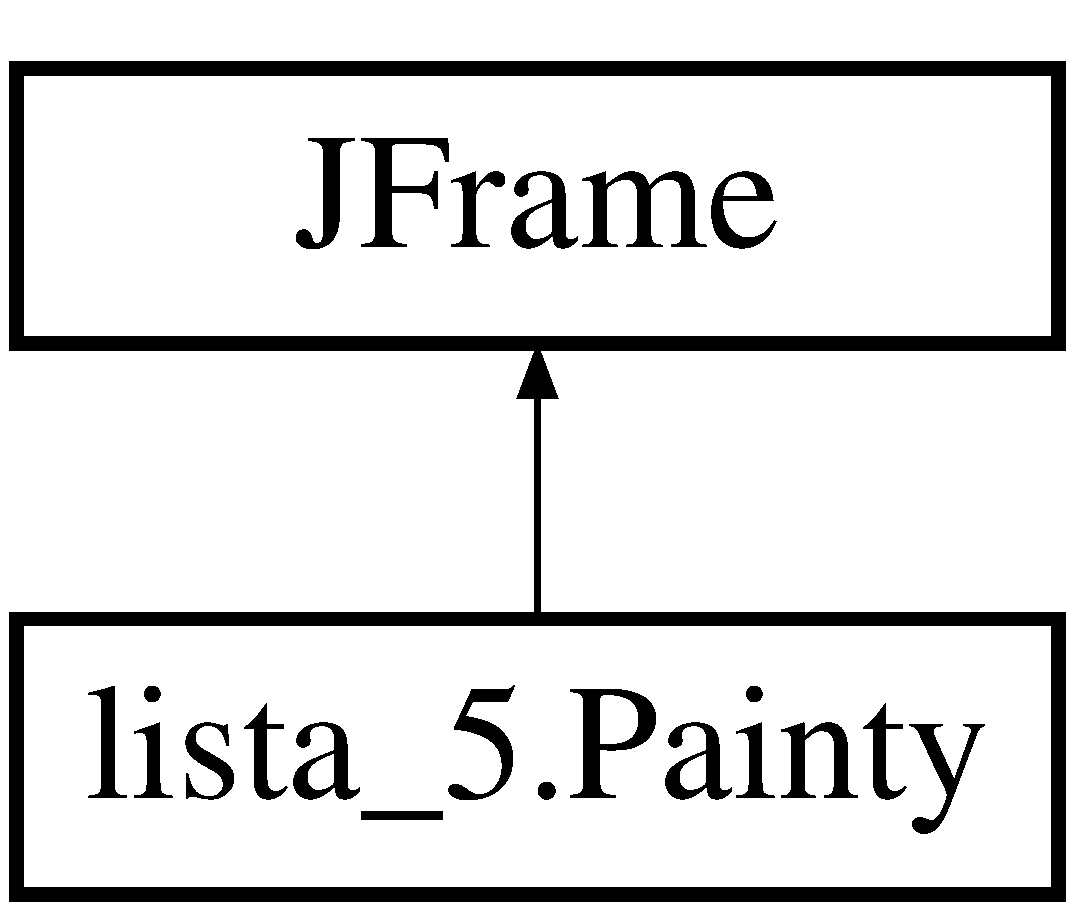
\includegraphics[height=2.000000cm]{classlista__5_1_1_painty}
\end{center}
\end{figure}
\subsection*{Public Member Functions}
\begin{DoxyCompactItemize}
\item 
\mbox{\hyperlink{classlista__5_1_1_painty_a71b4b4d6f8515244d5bd42fe8673d5fd}{Painty}} ()
\end{DoxyCompactItemize}
\subsection*{Static Public Member Functions}
\begin{DoxyCompactItemize}
\item 
static void \mbox{\hyperlink{classlista__5_1_1_painty_a95e397e2f87f16ee08fae4bbf926635e}{main}} (String\mbox{[}$\,$\mbox{]} args)
\end{DoxyCompactItemize}


\subsection{Detailed Description}
Glowna klasa programu graficznego. Wiecej informacji ogolnych\+: \begin{DoxySeeAlso}{See also}
\mbox{\hyperlink{classlista__5_1_1_info}{Info}} 
\end{DoxySeeAlso}
\begin{DoxyAuthor}{Author}
Piotr Andrzejewski 
\end{DoxyAuthor}
\begin{DoxyVersion}{Version}
3.\+2 
\end{DoxyVersion}


\subsection{Constructor \& Destructor Documentation}
\mbox{\Hypertarget{classlista__5_1_1_painty_a71b4b4d6f8515244d5bd42fe8673d5fd}\label{classlista__5_1_1_painty_a71b4b4d6f8515244d5bd42fe8673d5fd}} 
\index{lista\+\_\+5\+::\+Painty@{lista\+\_\+5\+::\+Painty}!Painty@{Painty}}
\index{Painty@{Painty}!lista\+\_\+5\+::\+Painty@{lista\+\_\+5\+::\+Painty}}
\subsubsection{\texorpdfstring{Painty()}{Painty()}}
{\footnotesize\ttfamily lista\+\_\+5.\+Painty.\+Painty (\begin{DoxyParamCaption}{ }\end{DoxyParamCaption})}



\subsection{Member Function Documentation}
\mbox{\Hypertarget{classlista__5_1_1_painty_a95e397e2f87f16ee08fae4bbf926635e}\label{classlista__5_1_1_painty_a95e397e2f87f16ee08fae4bbf926635e}} 
\index{lista\+\_\+5\+::\+Painty@{lista\+\_\+5\+::\+Painty}!main@{main}}
\index{main@{main}!lista\+\_\+5\+::\+Painty@{lista\+\_\+5\+::\+Painty}}
\subsubsection{\texorpdfstring{main()}{main()}}
{\footnotesize\ttfamily static void lista\+\_\+5.\+Painty.\+main (\begin{DoxyParamCaption}\item[{String \mbox{[}$\,$\mbox{]}}]{args }\end{DoxyParamCaption})\hspace{0.3cm}{\ttfamily [static]}}



The documentation for this class was generated from the following file\+:\begin{DoxyCompactItemize}
\item 
lista\+\_\+5/\mbox{\hyperlink{_painty_8java}{Painty.\+java}}\end{DoxyCompactItemize}

\hypertarget{classlista__5_1_1_prawy_bok}{}\section{lista\+\_\+5.\+Prawy\+Bok Class Reference}
\label{classlista__5_1_1_prawy_bok}\index{lista\+\_\+5.\+Prawy\+Bok@{lista\+\_\+5.\+Prawy\+Bok}}
Inheritance diagram for lista\+\_\+5.\+Prawy\+Bok\+:\begin{figure}[H]
\begin{center}
\leavevmode
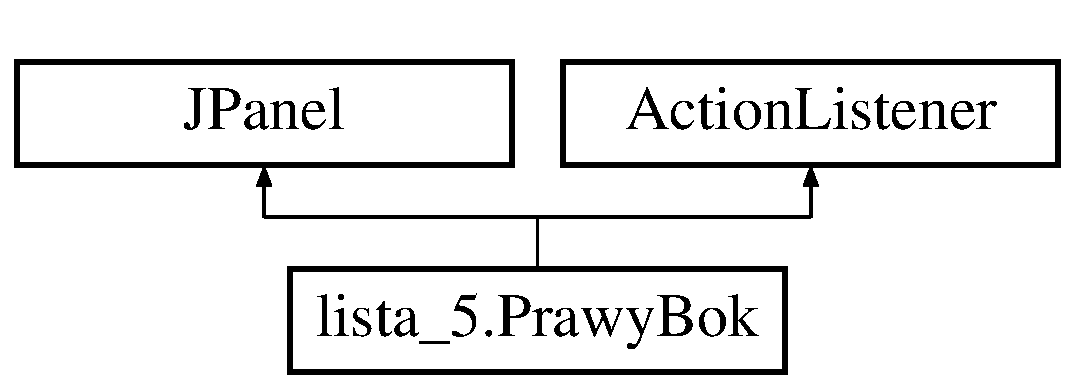
\includegraphics[height=2.000000cm]{classlista__5_1_1_prawy_bok}
\end{center}
\end{figure}
\subsection*{Public Member Functions}
\begin{DoxyCompactItemize}
\item 
\mbox{\hyperlink{classlista__5_1_1_prawy_bok_af7872920a7b9440729c7321e98b62de3}{Prawy\+Bok}} (\mbox{\hyperlink{classlista__5_1_1_wnetrze}{Wnetrze}} \mbox{\hyperlink{classlista__5_1_1_prawy_bok_a78d3ca2516dbab20a29c94c57b83c071}{wnetrze}})
\item 
void \mbox{\hyperlink{classlista__5_1_1_prawy_bok_a8966b8a4e49226ba2116a33c07f3060b}{action\+Performed}} (Action\+Event e)
\end{DoxyCompactItemize}
\subsection*{Static Package Attributes}
\begin{DoxyCompactItemize}
\item 
static J\+Toggle\+Button \mbox{\hyperlink{classlista__5_1_1_prawy_bok_a3d4126ae2e2d5d34dcd1d1dcc7300c85}{tworz}}
\item 
static J\+Toggle\+Button \mbox{\hyperlink{classlista__5_1_1_prawy_bok_ad7381fade3bbf8ffd8a5ad75a7b1f536}{kolo}}
\item 
static J\+Toggle\+Button \mbox{\hyperlink{classlista__5_1_1_prawy_bok_a36967d5d6c89e8b3ed3cf959869865a6}{prostokat}}
\item 
static J\+Toggle\+Button \mbox{\hyperlink{classlista__5_1_1_prawy_bok_ad6cb894230f53ab9e8ccdcab78d3b779}{wielokat}}
\item 
static J\+Toggle\+Button \mbox{\hyperlink{classlista__5_1_1_prawy_bok_afa582913eae025c445b56350c50e2bcf}{modyfikuj}}
\end{DoxyCompactItemize}
\subsection*{Private Attributes}
\begin{DoxyCompactItemize}
\item 
J\+Panel \mbox{\hyperlink{classlista__5_1_1_prawy_bok_a5835844758db5e5e2e7ab2abcde758a9}{figury}}
\item 
\mbox{\hyperlink{classlista__5_1_1_wnetrze}{Wnetrze}} \mbox{\hyperlink{classlista__5_1_1_prawy_bok_a78d3ca2516dbab20a29c94c57b83c071}{wnetrze}}
\end{DoxyCompactItemize}


\subsection{Detailed Description}
Panel po prawej strony, zawierający przyciski służące do tworzenia i edycji figur. 

\subsection{Constructor \& Destructor Documentation}
\mbox{\Hypertarget{classlista__5_1_1_prawy_bok_af7872920a7b9440729c7321e98b62de3}\label{classlista__5_1_1_prawy_bok_af7872920a7b9440729c7321e98b62de3}} 
\index{lista\+\_\+5\+::\+Prawy\+Bok@{lista\+\_\+5\+::\+Prawy\+Bok}!Prawy\+Bok@{Prawy\+Bok}}
\index{Prawy\+Bok@{Prawy\+Bok}!lista\+\_\+5\+::\+Prawy\+Bok@{lista\+\_\+5\+::\+Prawy\+Bok}}
\subsubsection{\texorpdfstring{Prawy\+Bok()}{PrawyBok()}}
{\footnotesize\ttfamily lista\+\_\+5.\+Prawy\+Bok.\+Prawy\+Bok (\begin{DoxyParamCaption}\item[{\mbox{\hyperlink{classlista__5_1_1_wnetrze}{Wnetrze}}}]{wnetrze }\end{DoxyParamCaption})}

Powołuje do życia obiekty, ustawia wygląd przycisków i całego panelu. 
\begin{DoxyParams}{Parameters}
{\em wnetrze} & panel, na którym rysujemy \\
\hline
\end{DoxyParams}


\subsection{Member Function Documentation}
\mbox{\Hypertarget{classlista__5_1_1_prawy_bok_a8966b8a4e49226ba2116a33c07f3060b}\label{classlista__5_1_1_prawy_bok_a8966b8a4e49226ba2116a33c07f3060b}} 
\index{lista\+\_\+5\+::\+Prawy\+Bok@{lista\+\_\+5\+::\+Prawy\+Bok}!action\+Performed@{action\+Performed}}
\index{action\+Performed@{action\+Performed}!lista\+\_\+5\+::\+Prawy\+Bok@{lista\+\_\+5\+::\+Prawy\+Bok}}
\subsubsection{\texorpdfstring{action\+Performed()}{actionPerformed()}}
{\footnotesize\ttfamily void lista\+\_\+5.\+Prawy\+Bok.\+action\+Performed (\begin{DoxyParamCaption}\item[{Action\+Event}]{e }\end{DoxyParamCaption})}

Obsługuje wszystkie zdarzenia związane z klikaniem i odklikaniem przycisków. Wywołuje także metodę \mbox{\hyperlink{classlista__5_1_1_wnetrze_aa5e96d1ba61b233b93c6d8a71931be07}{Wnetrze\#usun\+Wielokat()}}, jeśli ktoś zmienia tryb przed skończeniem rysowania.


\begin{DoxyParams}{Parameters}
{\em e} & zdarzenie -\/ kliknięcie któregoś z przycisków \\
\hline
\end{DoxyParams}


\subsection{Member Data Documentation}
\mbox{\Hypertarget{classlista__5_1_1_prawy_bok_a5835844758db5e5e2e7ab2abcde758a9}\label{classlista__5_1_1_prawy_bok_a5835844758db5e5e2e7ab2abcde758a9}} 
\index{lista\+\_\+5\+::\+Prawy\+Bok@{lista\+\_\+5\+::\+Prawy\+Bok}!figury@{figury}}
\index{figury@{figury}!lista\+\_\+5\+::\+Prawy\+Bok@{lista\+\_\+5\+::\+Prawy\+Bok}}
\subsubsection{\texorpdfstring{figury}{figury}}
{\footnotesize\ttfamily J\+Panel lista\+\_\+5.\+Prawy\+Bok.\+figury\hspace{0.3cm}{\ttfamily [private]}}

Panel, w którym przechowywane są przyciski odpowiadające za tworzenie poszczegolnych figur -\/ kolo, prostokat i wielokat. \mbox{\Hypertarget{classlista__5_1_1_prawy_bok_ad7381fade3bbf8ffd8a5ad75a7b1f536}\label{classlista__5_1_1_prawy_bok_ad7381fade3bbf8ffd8a5ad75a7b1f536}} 
\index{lista\+\_\+5\+::\+Prawy\+Bok@{lista\+\_\+5\+::\+Prawy\+Bok}!kolo@{kolo}}
\index{kolo@{kolo}!lista\+\_\+5\+::\+Prawy\+Bok@{lista\+\_\+5\+::\+Prawy\+Bok}}
\subsubsection{\texorpdfstring{kolo}{kolo}}
{\footnotesize\ttfamily J\+Toggle\+Button lista\+\_\+5.\+Prawy\+Bok.\+kolo\hspace{0.3cm}{\ttfamily [static]}, {\ttfamily [package]}}

Przycisk, który przełącza program w tryb tworzenia koła. \mbox{\Hypertarget{classlista__5_1_1_prawy_bok_afa582913eae025c445b56350c50e2bcf}\label{classlista__5_1_1_prawy_bok_afa582913eae025c445b56350c50e2bcf}} 
\index{lista\+\_\+5\+::\+Prawy\+Bok@{lista\+\_\+5\+::\+Prawy\+Bok}!modyfikuj@{modyfikuj}}
\index{modyfikuj@{modyfikuj}!lista\+\_\+5\+::\+Prawy\+Bok@{lista\+\_\+5\+::\+Prawy\+Bok}}
\subsubsection{\texorpdfstring{modyfikuj}{modyfikuj}}
{\footnotesize\ttfamily J\+Toggle\+Button lista\+\_\+5.\+Prawy\+Bok.\+modyfikuj\hspace{0.3cm}{\ttfamily [static]}, {\ttfamily [package]}}

Przycisk, który przełącza program w tryb edycji. \mbox{\Hypertarget{classlista__5_1_1_prawy_bok_a36967d5d6c89e8b3ed3cf959869865a6}\label{classlista__5_1_1_prawy_bok_a36967d5d6c89e8b3ed3cf959869865a6}} 
\index{lista\+\_\+5\+::\+Prawy\+Bok@{lista\+\_\+5\+::\+Prawy\+Bok}!prostokat@{prostokat}}
\index{prostokat@{prostokat}!lista\+\_\+5\+::\+Prawy\+Bok@{lista\+\_\+5\+::\+Prawy\+Bok}}
\subsubsection{\texorpdfstring{prostokat}{prostokat}}
{\footnotesize\ttfamily J\+Toggle\+Button lista\+\_\+5.\+Prawy\+Bok.\+prostokat\hspace{0.3cm}{\ttfamily [static]}, {\ttfamily [package]}}

Przycisk, który przełącza program w tryb tworzenia prostokąta. \mbox{\Hypertarget{classlista__5_1_1_prawy_bok_a3d4126ae2e2d5d34dcd1d1dcc7300c85}\label{classlista__5_1_1_prawy_bok_a3d4126ae2e2d5d34dcd1d1dcc7300c85}} 
\index{lista\+\_\+5\+::\+Prawy\+Bok@{lista\+\_\+5\+::\+Prawy\+Bok}!tworz@{tworz}}
\index{tworz@{tworz}!lista\+\_\+5\+::\+Prawy\+Bok@{lista\+\_\+5\+::\+Prawy\+Bok}}
\subsubsection{\texorpdfstring{tworz}{tworz}}
{\footnotesize\ttfamily J\+Toggle\+Button lista\+\_\+5.\+Prawy\+Bok.\+tworz\hspace{0.3cm}{\ttfamily [static]}, {\ttfamily [package]}}

Przycisk, który przełącza program w tryb tworzenia. \mbox{\Hypertarget{classlista__5_1_1_prawy_bok_ad6cb894230f53ab9e8ccdcab78d3b779}\label{classlista__5_1_1_prawy_bok_ad6cb894230f53ab9e8ccdcab78d3b779}} 
\index{lista\+\_\+5\+::\+Prawy\+Bok@{lista\+\_\+5\+::\+Prawy\+Bok}!wielokat@{wielokat}}
\index{wielokat@{wielokat}!lista\+\_\+5\+::\+Prawy\+Bok@{lista\+\_\+5\+::\+Prawy\+Bok}}
\subsubsection{\texorpdfstring{wielokat}{wielokat}}
{\footnotesize\ttfamily J\+Toggle\+Button lista\+\_\+5.\+Prawy\+Bok.\+wielokat\hspace{0.3cm}{\ttfamily [static]}, {\ttfamily [package]}}

Przycisk, który przełącza program w tryb tworzenia wielokąta. \mbox{\Hypertarget{classlista__5_1_1_prawy_bok_a78d3ca2516dbab20a29c94c57b83c071}\label{classlista__5_1_1_prawy_bok_a78d3ca2516dbab20a29c94c57b83c071}} 
\index{lista\+\_\+5\+::\+Prawy\+Bok@{lista\+\_\+5\+::\+Prawy\+Bok}!wnetrze@{wnetrze}}
\index{wnetrze@{wnetrze}!lista\+\_\+5\+::\+Prawy\+Bok@{lista\+\_\+5\+::\+Prawy\+Bok}}
\subsubsection{\texorpdfstring{wnetrze}{wnetrze}}
{\footnotesize\ttfamily \mbox{\hyperlink{classlista__5_1_1_wnetrze}{Wnetrze}} lista\+\_\+5.\+Prawy\+Bok.\+wnetrze\hspace{0.3cm}{\ttfamily [private]}}

Odpowiada panelowi Wnętrze, potrzebujemy to pole w celu wywołania metod \mbox{\hyperlink{classlista__5_1_1_wnetrze_aa5e96d1ba61b233b93c6d8a71931be07}{Wnetrze\#usun\+Wielokat()}}; 

The documentation for this class was generated from the following file\+:\begin{DoxyCompactItemize}
\item 
lista\+\_\+5/\mbox{\hyperlink{_prawy_bok_8java}{Prawy\+Bok.\+java}}\end{DoxyCompactItemize}

\hypertarget{classlista__5_1_1_prostokat}{}\section{lista\+\_\+5.\+Prostokat Class Reference}
\label{classlista__5_1_1_prostokat}\index{lista\+\_\+5.\+Prostokat@{lista\+\_\+5.\+Prostokat}}
Inheritance diagram for lista\+\_\+5.\+Prostokat\+:\begin{figure}[H]
\begin{center}
\leavevmode
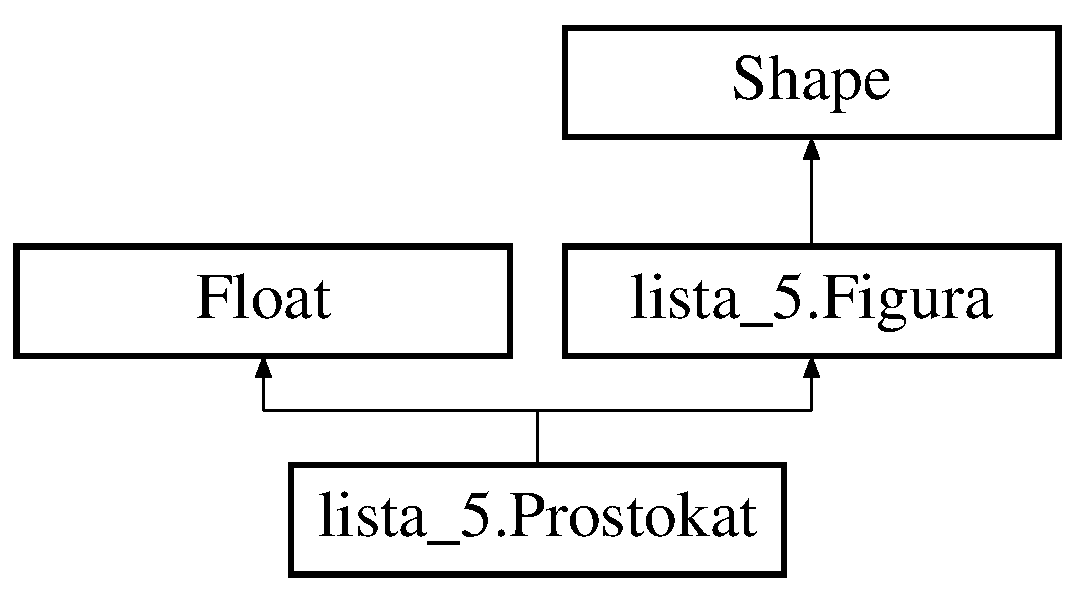
\includegraphics[height=3.000000cm]{classlista__5_1_1_prostokat}
\end{center}
\end{figure}
\subsection*{Public Member Functions}
\begin{DoxyCompactItemize}
\item 
\mbox{\hyperlink{classlista__5_1_1_prostokat_acc8c546649b600148d733120799f0df6}{Prostokat}} (Point d)
\item 
void \mbox{\hyperlink{classlista__5_1_1_prostokat_a63b2bb7a2b3fd86e21d0d125f4262f39}{rysuj}} (Point zmienny)
\item 
void \mbox{\hyperlink{classlista__5_1_1_prostokat_a9e8a5112287441debbfe24165a24d322}{przesun}} (int dx, int dy)
\item 
void \mbox{\hyperlink{classlista__5_1_1_prostokat_acc961816d5fba86f3442ca34059492f5}{zwieksz}} (int zwiekszenie)
\item 
void \mbox{\hyperlink{classlista__5_1_1_prostokat_a95b9ce7b2a7b095c43ffc843cfeff39a}{wypisz\+Dane}} ()
\item 
String \mbox{\hyperlink{classlista__5_1_1_prostokat_a9537add38b8302420692068fb36726b5}{zapisz\+Dane}} ()
\item 
void \mbox{\hyperlink{classlista__5_1_1_prostokat_a93ae9f652ca00886c05be661b17a0886}{ustaw\+Z\+Odczytu}} (String\mbox{[}$\,$\mbox{]} argumenty)
\item 
void \mbox{\hyperlink{classlista__5_1_1_prostokat_aa776fbd55cc88f2bb8b8a202109e77ce}{zmien\+Kolor}} (Graphics2D g2d, Color \mbox{\hyperlink{classlista__5_1_1_prostokat_ad4564e93752646ac3267d2f559c25907}{kolor}})
\item 
void \mbox{\hyperlink{classlista__5_1_1_prostokat_ad63e4a8c7f291a54f8c9c285c8e6c8ff}{ustaw\+Kolor}} (Graphics2D g2d)
\end{DoxyCompactItemize}
\subsection*{Private Attributes}
\begin{DoxyCompactItemize}
\item 
Point \mbox{\hyperlink{classlista__5_1_1_prostokat_adde334d6e8c665362e02745b04bec40d}{wyjsciowy}}
\item 
Color \mbox{\hyperlink{classlista__5_1_1_prostokat_ad4564e93752646ac3267d2f559c25907}{kolor}} = Color.\+O\+R\+A\+N\+GE
\item 
final int \mbox{\hyperlink{classlista__5_1_1_prostokat_a091fff7a1557fe594f834863d888be0c}{min\+\_\+width}} = 20
\item 
final int \mbox{\hyperlink{classlista__5_1_1_prostokat_acf9d581dee47e46a8139bda38d1993d6}{min\+\_\+height}} = 20
\end{DoxyCompactItemize}


\subsection{Detailed Description}
Klasa reprezentująca prostokąt. \begin{DoxySeeAlso}{See also}
\mbox{\hyperlink{interfacelista__5_1_1_figura}{Figura}} 
\end{DoxySeeAlso}


\subsection{Constructor \& Destructor Documentation}
\mbox{\Hypertarget{classlista__5_1_1_prostokat_acc8c546649b600148d733120799f0df6}\label{classlista__5_1_1_prostokat_acc8c546649b600148d733120799f0df6}} 
\index{lista\+\_\+5\+::\+Prostokat@{lista\+\_\+5\+::\+Prostokat}!Prostokat@{Prostokat}}
\index{Prostokat@{Prostokat}!lista\+\_\+5\+::\+Prostokat@{lista\+\_\+5\+::\+Prostokat}}
\subsubsection{\texorpdfstring{Prostokat()}{Prostokat()}}
{\footnotesize\ttfamily lista\+\_\+5.\+Prostokat.\+Prostokat (\begin{DoxyParamCaption}\item[{Point}]{d }\end{DoxyParamCaption})}

Tworzy \mbox{\hyperlink{classlista__5_1_1_prostokat}{Prostokat}}, ustalając współrzędne punktu wyjsciowego. 
\begin{DoxyParams}{Parameters}
{\em d} & punkt wyjściowy \\
\hline
\end{DoxyParams}
\begin{DoxySeeAlso}{See also}
\mbox{\hyperlink{classlista__5_1_1_prostokat_adde334d6e8c665362e02745b04bec40d}{wyjsciowy}} 
\end{DoxySeeAlso}


\subsection{Member Function Documentation}
\mbox{\Hypertarget{classlista__5_1_1_prostokat_a9e8a5112287441debbfe24165a24d322}\label{classlista__5_1_1_prostokat_a9e8a5112287441debbfe24165a24d322}} 
\index{lista\+\_\+5\+::\+Prostokat@{lista\+\_\+5\+::\+Prostokat}!przesun@{przesun}}
\index{przesun@{przesun}!lista\+\_\+5\+::\+Prostokat@{lista\+\_\+5\+::\+Prostokat}}
\subsubsection{\texorpdfstring{przesun()}{przesun()}}
{\footnotesize\ttfamily void lista\+\_\+5.\+Prostokat.\+przesun (\begin{DoxyParamCaption}\item[{int}]{dx,  }\item[{int}]{dy }\end{DoxyParamCaption})}

Zmienia położenie figury. 
\begin{DoxyParams}{Parameters}
{\em dx} & zmiana położenia względem osi x, o którą należy przesunąć figurę \\
\hline
{\em dy} & zmiana położenia względem osi y, o którą należy przesunąć figurę\\
\hline
\end{DoxyParams}
 

Implements \mbox{\hyperlink{interfacelista__5_1_1_figura_a72f085618cf604e8b1632ea733043861}{lista\+\_\+5.\+Figura}}.

\mbox{\Hypertarget{classlista__5_1_1_prostokat_a63b2bb7a2b3fd86e21d0d125f4262f39}\label{classlista__5_1_1_prostokat_a63b2bb7a2b3fd86e21d0d125f4262f39}} 
\index{lista\+\_\+5\+::\+Prostokat@{lista\+\_\+5\+::\+Prostokat}!rysuj@{rysuj}}
\index{rysuj@{rysuj}!lista\+\_\+5\+::\+Prostokat@{lista\+\_\+5\+::\+Prostokat}}
\subsubsection{\texorpdfstring{rysuj()}{rysuj()}}
{\footnotesize\ttfamily void lista\+\_\+5.\+Prostokat.\+rysuj (\begin{DoxyParamCaption}\item[{Point}]{zmienny }\end{DoxyParamCaption})}

Zmienia właściwości figury podczas jej tworzenia i rysowania; 
\begin{DoxyParams}{Parameters}
{\em d} & nowy
\begin{DoxyCode}
Point 
\end{DoxyCode}
 , który zmienia kształt figury\\
\hline
\end{DoxyParams}
 
\begin{DoxyParams}{Parameters}
{\em zmienny} & prawy dolny róg prostokąta \\
\hline
\end{DoxyParams}


Implements \mbox{\hyperlink{interfacelista__5_1_1_figura_a1b238957bac675c57febc970067dfd6d}{lista\+\_\+5.\+Figura}}.

\mbox{\Hypertarget{classlista__5_1_1_prostokat_ad63e4a8c7f291a54f8c9c285c8e6c8ff}\label{classlista__5_1_1_prostokat_ad63e4a8c7f291a54f8c9c285c8e6c8ff}} 
\index{lista\+\_\+5\+::\+Prostokat@{lista\+\_\+5\+::\+Prostokat}!ustaw\+Kolor@{ustaw\+Kolor}}
\index{ustaw\+Kolor@{ustaw\+Kolor}!lista\+\_\+5\+::\+Prostokat@{lista\+\_\+5\+::\+Prostokat}}
\subsubsection{\texorpdfstring{ustaw\+Kolor()}{ustawKolor()}}
{\footnotesize\ttfamily void lista\+\_\+5.\+Prostokat.\+ustaw\+Kolor (\begin{DoxyParamCaption}\item[{Graphics2D}]{g2d }\end{DoxyParamCaption})}

Zmienia kolor grafiki na ten, który jest przechowywane w polu kolor. 
\begin{DoxyParams}{Parameters}
{\em g2d} & grafika używana w \mbox{\hyperlink{classlista__5_1_1_wnetrze_aa8676192e150a17230d72de122744a47}{Wnetrze\#paint\+Component}} \\
\hline
\end{DoxyParams}
\begin{DoxySeeAlso}{See also}
\mbox{\hyperlink{interfacelista__5_1_1_figura_aeb0982dc44348dd1fde9266d9d476ed0}{zmien\+Kolor}}
\end{DoxySeeAlso}
 

Implements \mbox{\hyperlink{interfacelista__5_1_1_figura_a3cc13bf7229b288d743be7903b3b61a4}{lista\+\_\+5.\+Figura}}.

\mbox{\Hypertarget{classlista__5_1_1_prostokat_a93ae9f652ca00886c05be661b17a0886}\label{classlista__5_1_1_prostokat_a93ae9f652ca00886c05be661b17a0886}} 
\index{lista\+\_\+5\+::\+Prostokat@{lista\+\_\+5\+::\+Prostokat}!ustaw\+Z\+Odczytu@{ustaw\+Z\+Odczytu}}
\index{ustaw\+Z\+Odczytu@{ustaw\+Z\+Odczytu}!lista\+\_\+5\+::\+Prostokat@{lista\+\_\+5\+::\+Prostokat}}
\subsubsection{\texorpdfstring{ustaw\+Z\+Odczytu()}{ustawZOdczytu()}}
{\footnotesize\ttfamily void lista\+\_\+5.\+Prostokat.\+ustaw\+Z\+Odczytu (\begin{DoxyParamCaption}\item[{String \mbox{[}$\,$\mbox{]}}]{argumenty }\end{DoxyParamCaption})}

Ustawia całą figurę korzystając z danych z pliku. 
\begin{DoxyParams}{Parameters}
{\em argumenty} & tablica danych z odczytu, zawiera informacje determinujące figurę\\
\hline
\end{DoxyParams}
 

Implements \mbox{\hyperlink{interfacelista__5_1_1_figura_a75b72b51014348d839e1f2b81525f264}{lista\+\_\+5.\+Figura}}.

\mbox{\Hypertarget{classlista__5_1_1_prostokat_a95b9ce7b2a7b095c43ffc843cfeff39a}\label{classlista__5_1_1_prostokat_a95b9ce7b2a7b095c43ffc843cfeff39a}} 
\index{lista\+\_\+5\+::\+Prostokat@{lista\+\_\+5\+::\+Prostokat}!wypisz\+Dane@{wypisz\+Dane}}
\index{wypisz\+Dane@{wypisz\+Dane}!lista\+\_\+5\+::\+Prostokat@{lista\+\_\+5\+::\+Prostokat}}
\subsubsection{\texorpdfstring{wypisz\+Dane()}{wypiszDane()}}
{\footnotesize\ttfamily void lista\+\_\+5.\+Prostokat.\+wypisz\+Dane (\begin{DoxyParamCaption}{ }\end{DoxyParamCaption})}

Wypisuje dane związane z figurą w \mbox{\hyperlink{classlista__5_1_1_stopka_a8e8ef21758defd5b137e609b00d2f59e}{Stopka\#dane}} 

Implements \mbox{\hyperlink{interfacelista__5_1_1_figura_aaddd90c61fd1632655cb031efafe1a7d}{lista\+\_\+5.\+Figura}}.

\mbox{\Hypertarget{classlista__5_1_1_prostokat_a9537add38b8302420692068fb36726b5}\label{classlista__5_1_1_prostokat_a9537add38b8302420692068fb36726b5}} 
\index{lista\+\_\+5\+::\+Prostokat@{lista\+\_\+5\+::\+Prostokat}!zapisz\+Dane@{zapisz\+Dane}}
\index{zapisz\+Dane@{zapisz\+Dane}!lista\+\_\+5\+::\+Prostokat@{lista\+\_\+5\+::\+Prostokat}}
\subsubsection{\texorpdfstring{zapisz\+Dane()}{zapiszDane()}}
{\footnotesize\ttfamily String lista\+\_\+5.\+Prostokat.\+zapisz\+Dane (\begin{DoxyParamCaption}{ }\end{DoxyParamCaption})}

Przygotowuje informacje o figurze do zapisania. \begin{DoxyReturn}{Returns}
linia, która zostanie zapisana w pliku
\end{DoxyReturn}
 

Implements \mbox{\hyperlink{interfacelista__5_1_1_figura_a9d60d64b495755a3e48a3eee549a728d}{lista\+\_\+5.\+Figura}}.

\mbox{\Hypertarget{classlista__5_1_1_prostokat_aa776fbd55cc88f2bb8b8a202109e77ce}\label{classlista__5_1_1_prostokat_aa776fbd55cc88f2bb8b8a202109e77ce}} 
\index{lista\+\_\+5\+::\+Prostokat@{lista\+\_\+5\+::\+Prostokat}!zmien\+Kolor@{zmien\+Kolor}}
\index{zmien\+Kolor@{zmien\+Kolor}!lista\+\_\+5\+::\+Prostokat@{lista\+\_\+5\+::\+Prostokat}}
\subsubsection{\texorpdfstring{zmien\+Kolor()}{zmienKolor()}}
{\footnotesize\ttfamily void lista\+\_\+5.\+Prostokat.\+zmien\+Kolor (\begin{DoxyParamCaption}\item[{Graphics2D}]{g2d,  }\item[{Color}]{kolor }\end{DoxyParamCaption})}

Aktualizuje pole kolor obecne w każdej figurze. 
\begin{DoxyParams}{Parameters}
{\em g2d} & grafika używana w \mbox{\hyperlink{classlista__5_1_1_wnetrze_aa8676192e150a17230d72de122744a47}{Wnetrze\#paint\+Component}} \\
\hline
{\em kolor} & pożądany kolor \\
\hline
\end{DoxyParams}
\begin{DoxySeeAlso}{See also}
\mbox{\hyperlink{interfacelista__5_1_1_figura_a3cc13bf7229b288d743be7903b3b61a4}{ustaw\+Kolor}}
\end{DoxySeeAlso}
 

Implements \mbox{\hyperlink{interfacelista__5_1_1_figura_aeb0982dc44348dd1fde9266d9d476ed0}{lista\+\_\+5.\+Figura}}.

\mbox{\Hypertarget{classlista__5_1_1_prostokat_acc961816d5fba86f3442ca34059492f5}\label{classlista__5_1_1_prostokat_acc961816d5fba86f3442ca34059492f5}} 
\index{lista\+\_\+5\+::\+Prostokat@{lista\+\_\+5\+::\+Prostokat}!zwieksz@{zwieksz}}
\index{zwieksz@{zwieksz}!lista\+\_\+5\+::\+Prostokat@{lista\+\_\+5\+::\+Prostokat}}
\subsubsection{\texorpdfstring{zwieksz()}{zwieksz()}}
{\footnotesize\ttfamily void lista\+\_\+5.\+Prostokat.\+zwieksz (\begin{DoxyParamCaption}\item[{int}]{zwiekszenie }\end{DoxyParamCaption})}

Powiększa rozmiary figury. 
\begin{DoxyParams}{Parameters}
{\em zwiekszenie} & wartość, o którą należy zwiększyć figurę przy skalowaniu\\
\hline
\end{DoxyParams}
, pamiętając o wartościach minimalnych. \begin{DoxySeeAlso}{See also}
\mbox{\hyperlink{classlista__5_1_1_prostokat_a091fff7a1557fe594f834863d888be0c}{min\+\_\+width}} 

\mbox{\hyperlink{classlista__5_1_1_prostokat_acf9d581dee47e46a8139bda38d1993d6}{min\+\_\+height}} 
\end{DoxySeeAlso}


Implements \mbox{\hyperlink{interfacelista__5_1_1_figura_a6813d7ac31e5118bcb34b9b29868ce5f}{lista\+\_\+5.\+Figura}}.



\subsection{Member Data Documentation}
\mbox{\Hypertarget{classlista__5_1_1_prostokat_ad4564e93752646ac3267d2f559c25907}\label{classlista__5_1_1_prostokat_ad4564e93752646ac3267d2f559c25907}} 
\index{lista\+\_\+5\+::\+Prostokat@{lista\+\_\+5\+::\+Prostokat}!kolor@{kolor}}
\index{kolor@{kolor}!lista\+\_\+5\+::\+Prostokat@{lista\+\_\+5\+::\+Prostokat}}
\subsubsection{\texorpdfstring{kolor}{kolor}}
{\footnotesize\ttfamily Color lista\+\_\+5.\+Prostokat.\+kolor = Color.\+O\+R\+A\+N\+GE\hspace{0.3cm}{\ttfamily [private]}}


\begin{DoxyCode}
Color 
\end{DoxyCode}
 , domyślnie ustawiony na
\begin{DoxyCode}
Color.ORANGE 
\end{DoxyCode}
 \mbox{\Hypertarget{classlista__5_1_1_prostokat_acf9d581dee47e46a8139bda38d1993d6}\label{classlista__5_1_1_prostokat_acf9d581dee47e46a8139bda38d1993d6}} 
\index{lista\+\_\+5\+::\+Prostokat@{lista\+\_\+5\+::\+Prostokat}!min\+\_\+height@{min\+\_\+height}}
\index{min\+\_\+height@{min\+\_\+height}!lista\+\_\+5\+::\+Prostokat@{lista\+\_\+5\+::\+Prostokat}}
\subsubsection{\texorpdfstring{min\+\_\+height}{min\_height}}
{\footnotesize\ttfamily final int lista\+\_\+5.\+Prostokat.\+min\+\_\+height = 20\hspace{0.3cm}{\ttfamily [private]}}

Minimalna wysokość, która jest nieprzekraczalna przy zmniejszaniu. \mbox{\Hypertarget{classlista__5_1_1_prostokat_a091fff7a1557fe594f834863d888be0c}\label{classlista__5_1_1_prostokat_a091fff7a1557fe594f834863d888be0c}} 
\index{lista\+\_\+5\+::\+Prostokat@{lista\+\_\+5\+::\+Prostokat}!min\+\_\+width@{min\+\_\+width}}
\index{min\+\_\+width@{min\+\_\+width}!lista\+\_\+5\+::\+Prostokat@{lista\+\_\+5\+::\+Prostokat}}
\subsubsection{\texorpdfstring{min\+\_\+width}{min\_width}}
{\footnotesize\ttfamily final int lista\+\_\+5.\+Prostokat.\+min\+\_\+width = 20\hspace{0.3cm}{\ttfamily [private]}}

Minimalna szerokość, która jest nieprzekraczalna przy zmniejszaniu. \mbox{\Hypertarget{classlista__5_1_1_prostokat_adde334d6e8c665362e02745b04bec40d}\label{classlista__5_1_1_prostokat_adde334d6e8c665362e02745b04bec40d}} 
\index{lista\+\_\+5\+::\+Prostokat@{lista\+\_\+5\+::\+Prostokat}!wyjsciowy@{wyjsciowy}}
\index{wyjsciowy@{wyjsciowy}!lista\+\_\+5\+::\+Prostokat@{lista\+\_\+5\+::\+Prostokat}}
\subsubsection{\texorpdfstring{wyjsciowy}{wyjsciowy}}
{\footnotesize\ttfamily Point lista\+\_\+5.\+Prostokat.\+wyjsciowy\hspace{0.3cm}{\ttfamily [private]}}

wyjsciowy
\begin{DoxyCode}
Point 
\end{DoxyCode}
 , lewy górny róg prostokąta, niezmienny przy rysowaniu 

The documentation for this class was generated from the following file\+:\begin{DoxyCompactItemize}
\item 
lista\+\_\+5/\mbox{\hyperlink{_prostokat_8java}{Prostokat.\+java}}\end{DoxyCompactItemize}

\hypertarget{classlista__5_1_1_stopka}{}\section{lista\+\_\+5.\+Stopka Class Reference}
\label{classlista__5_1_1_stopka}\index{lista\+\_\+5.\+Stopka@{lista\+\_\+5.\+Stopka}}
Inheritance diagram for lista\+\_\+5.\+Stopka\+:\begin{figure}[H]
\begin{center}
\leavevmode
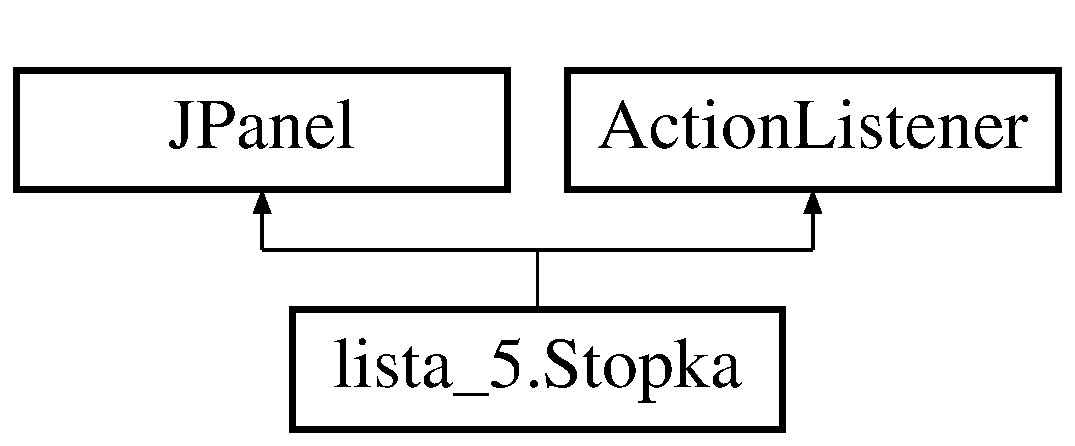
\includegraphics[height=2.000000cm]{classlista__5_1_1_stopka}
\end{center}
\end{figure}
\subsection*{Public Member Functions}
\begin{DoxyCompactItemize}
\item 
\mbox{\hyperlink{classlista__5_1_1_stopka_aca2946bc95b1b607793c5e57fc2ed995}{Stopka}} (\mbox{\hyperlink{classlista__5_1_1_wnetrze}{Wnetrze}} \mbox{\hyperlink{classlista__5_1_1_stopka_a047d15d43be6d71f8a27a3fa4528b272}{wnetrze}})
\item 
void \mbox{\hyperlink{classlista__5_1_1_stopka_a6cce6029ebcb4c780c78442687aadd8f}{action\+Performed}} (Action\+Event e)
\end{DoxyCompactItemize}
\subsection*{Static Package Attributes}
\begin{DoxyCompactItemize}
\item 
static J\+Text\+Area \mbox{\hyperlink{classlista__5_1_1_stopka_a8e8ef21758defd5b137e609b00d2f59e}{dane}}
\end{DoxyCompactItemize}
\subsection*{Private Attributes}
\begin{DoxyCompactItemize}
\item 
J\+Panel \mbox{\hyperlink{classlista__5_1_1_stopka_a5a1436f164fa7f3e65c148fb8716319f}{rog}}
\item 
J\+Button \mbox{\hyperlink{classlista__5_1_1_stopka_a77dc029a3ed5c0ea4d49b1279a01b1bc}{info}}
\item 
J\+Button \mbox{\hyperlink{classlista__5_1_1_stopka_a0086583a29887591d27fcfef4438b199}{zapisz}}
\item 
J\+Button \mbox{\hyperlink{classlista__5_1_1_stopka_a658e033afcd318e8f01051b5ff0caa0b}{odczyt}}
\item 
\mbox{\hyperlink{classlista__5_1_1_wnetrze}{Wnetrze}} \mbox{\hyperlink{classlista__5_1_1_stopka_a047d15d43be6d71f8a27a3fa4528b272}{wnetrze}}
\end{DoxyCompactItemize}


\subsection{Detailed Description}
Dolny panel panelu \mbox{\hyperlink{classlista__5_1_1_wyglad}{Wyglad}}. 

\subsection{Constructor \& Destructor Documentation}
\mbox{\Hypertarget{classlista__5_1_1_stopka_aca2946bc95b1b607793c5e57fc2ed995}\label{classlista__5_1_1_stopka_aca2946bc95b1b607793c5e57fc2ed995}} 
\index{lista\+\_\+5\+::\+Stopka@{lista\+\_\+5\+::\+Stopka}!Stopka@{Stopka}}
\index{Stopka@{Stopka}!lista\+\_\+5\+::\+Stopka@{lista\+\_\+5\+::\+Stopka}}
\subsubsection{\texorpdfstring{Stopka()}{Stopka()}}
{\footnotesize\ttfamily lista\+\_\+5.\+Stopka.\+Stopka (\begin{DoxyParamCaption}\item[{\mbox{\hyperlink{classlista__5_1_1_wnetrze}{Wnetrze}}}]{wnetrze }\end{DoxyParamCaption})}

Tworzymy stopkę, ustawiamy jej parametry i wygląd. 
\begin{DoxyParams}{Parameters}
{\em wnetrze} & panel, na którym rysujemy \\
\hline
\end{DoxyParams}


\subsection{Member Function Documentation}
\mbox{\Hypertarget{classlista__5_1_1_stopka_a6cce6029ebcb4c780c78442687aadd8f}\label{classlista__5_1_1_stopka_a6cce6029ebcb4c780c78442687aadd8f}} 
\index{lista\+\_\+5\+::\+Stopka@{lista\+\_\+5\+::\+Stopka}!action\+Performed@{action\+Performed}}
\index{action\+Performed@{action\+Performed}!lista\+\_\+5\+::\+Stopka@{lista\+\_\+5\+::\+Stopka}}
\subsubsection{\texorpdfstring{action\+Performed()}{actionPerformed()}}
{\footnotesize\ttfamily void lista\+\_\+5.\+Stopka.\+action\+Performed (\begin{DoxyParamCaption}\item[{Action\+Event}]{e }\end{DoxyParamCaption})}

Obsługuje zdarzenia, tworzy obiekt klasy \mbox{\hyperlink{classlista__5_1_1_info}{Info}}, uruchamia funkcję \mbox{\hyperlink{classlista__5_1_1_wnetrze_a3f2f50d048d7c41f2cbbb7f91f59c077}{Wnetrze\#zapisz()}} lub \mbox{\hyperlink{classlista__5_1_1_wnetrze_ad5ebd5c04f2c4b9de6954303c96a5856}{Wnetrze\#odczyt()}} (w zależności od zdarzenia). 
\begin{DoxyParams}{Parameters}
{\em e} & zdarzenie -\/ przyciśnięcie przycisku info, zapisz lub odczyt \\
\hline
\end{DoxyParams}
\begin{DoxySeeAlso}{See also}
\mbox{\hyperlink{classlista__5_1_1_wnetrze}{Wnetrze}} 
\end{DoxySeeAlso}


\subsection{Member Data Documentation}
\mbox{\Hypertarget{classlista__5_1_1_stopka_a8e8ef21758defd5b137e609b00d2f59e}\label{classlista__5_1_1_stopka_a8e8ef21758defd5b137e609b00d2f59e}} 
\index{lista\+\_\+5\+::\+Stopka@{lista\+\_\+5\+::\+Stopka}!dane@{dane}}
\index{dane@{dane}!lista\+\_\+5\+::\+Stopka@{lista\+\_\+5\+::\+Stopka}}
\subsubsection{\texorpdfstring{dane}{dane}}
{\footnotesize\ttfamily J\+Text\+Area lista\+\_\+5.\+Stopka.\+dane\hspace{0.3cm}{\ttfamily [static]}, {\ttfamily [package]}}

Miejsce, w którym wypisywane są informacje o figurze w trakcie przesuwania. \mbox{\Hypertarget{classlista__5_1_1_stopka_a77dc029a3ed5c0ea4d49b1279a01b1bc}\label{classlista__5_1_1_stopka_a77dc029a3ed5c0ea4d49b1279a01b1bc}} 
\index{lista\+\_\+5\+::\+Stopka@{lista\+\_\+5\+::\+Stopka}!info@{info}}
\index{info@{info}!lista\+\_\+5\+::\+Stopka@{lista\+\_\+5\+::\+Stopka}}
\subsubsection{\texorpdfstring{info}{info}}
{\footnotesize\ttfamily J\+Button lista\+\_\+5.\+Stopka.\+info\hspace{0.3cm}{\ttfamily [private]}}

Przycisk uruchamiający informacyjne okno dialogowe. \begin{DoxySeeAlso}{See also}
\mbox{\hyperlink{classlista__5_1_1_info}{Info}} 
\end{DoxySeeAlso}
\mbox{\Hypertarget{classlista__5_1_1_stopka_a658e033afcd318e8f01051b5ff0caa0b}\label{classlista__5_1_1_stopka_a658e033afcd318e8f01051b5ff0caa0b}} 
\index{lista\+\_\+5\+::\+Stopka@{lista\+\_\+5\+::\+Stopka}!odczyt@{odczyt}}
\index{odczyt@{odczyt}!lista\+\_\+5\+::\+Stopka@{lista\+\_\+5\+::\+Stopka}}
\subsubsection{\texorpdfstring{odczyt}{odczyt}}
{\footnotesize\ttfamily J\+Button lista\+\_\+5.\+Stopka.\+odczyt\hspace{0.3cm}{\ttfamily [private]}}

Przycisk rozpoczynający odczytywanie z pliku. \begin{DoxySeeAlso}{See also}
\mbox{\hyperlink{classlista__5_1_1_wnetrze_ad5ebd5c04f2c4b9de6954303c96a5856}{Wnetrze\+::odczyt()}} 
\end{DoxySeeAlso}
\mbox{\Hypertarget{classlista__5_1_1_stopka_a5a1436f164fa7f3e65c148fb8716319f}\label{classlista__5_1_1_stopka_a5a1436f164fa7f3e65c148fb8716319f}} 
\index{lista\+\_\+5\+::\+Stopka@{lista\+\_\+5\+::\+Stopka}!rog@{rog}}
\index{rog@{rog}!lista\+\_\+5\+::\+Stopka@{lista\+\_\+5\+::\+Stopka}}
\subsubsection{\texorpdfstring{rog}{rog}}
{\footnotesize\ttfamily J\+Panel lista\+\_\+5.\+Stopka.\+rog\hspace{0.3cm}{\ttfamily [private]}}

Panel z przyciskami, umieszczony w prawym dolnym rogu. \mbox{\Hypertarget{classlista__5_1_1_stopka_a047d15d43be6d71f8a27a3fa4528b272}\label{classlista__5_1_1_stopka_a047d15d43be6d71f8a27a3fa4528b272}} 
\index{lista\+\_\+5\+::\+Stopka@{lista\+\_\+5\+::\+Stopka}!wnetrze@{wnetrze}}
\index{wnetrze@{wnetrze}!lista\+\_\+5\+::\+Stopka@{lista\+\_\+5\+::\+Stopka}}
\subsubsection{\texorpdfstring{wnetrze}{wnetrze}}
{\footnotesize\ttfamily \mbox{\hyperlink{classlista__5_1_1_wnetrze}{Wnetrze}} lista\+\_\+5.\+Stopka.\+wnetrze\hspace{0.3cm}{\ttfamily [private]}}

Odpowiada panelowi Wnętrze, potrzebujemy to pole w celu wywołania metod \mbox{\hyperlink{classlista__5_1_1_stopka_a0086583a29887591d27fcfef4438b199}{zapisz}} i \mbox{\hyperlink{classlista__5_1_1_stopka_a658e033afcd318e8f01051b5ff0caa0b}{odczyt}}; \mbox{\Hypertarget{classlista__5_1_1_stopka_a0086583a29887591d27fcfef4438b199}\label{classlista__5_1_1_stopka_a0086583a29887591d27fcfef4438b199}} 
\index{lista\+\_\+5\+::\+Stopka@{lista\+\_\+5\+::\+Stopka}!zapisz@{zapisz}}
\index{zapisz@{zapisz}!lista\+\_\+5\+::\+Stopka@{lista\+\_\+5\+::\+Stopka}}
\subsubsection{\texorpdfstring{zapisz}{zapisz}}
{\footnotesize\ttfamily J\+Button lista\+\_\+5.\+Stopka.\+zapisz\hspace{0.3cm}{\ttfamily [private]}}

Przycisk rozpoczynający zapisywanie do pliku. \begin{DoxySeeAlso}{See also}
\mbox{\hyperlink{classlista__5_1_1_wnetrze_a3f2f50d048d7c41f2cbbb7f91f59c077}{Wnetrze\+::zapisz()}} 
\end{DoxySeeAlso}


The documentation for this class was generated from the following file\+:\begin{DoxyCompactItemize}
\item 
lista\+\_\+5/\mbox{\hyperlink{_stopka_8java}{Stopka.\+java}}\end{DoxyCompactItemize}

\hypertarget{classlista__5_1_1_wielokat}{}\section{lista\+\_\+5.\+Wielokat Class Reference}
\label{classlista__5_1_1_wielokat}\index{lista\+\_\+5.\+Wielokat@{lista\+\_\+5.\+Wielokat}}
Inheritance diagram for lista\+\_\+5.\+Wielokat\+:\begin{figure}[H]
\begin{center}
\leavevmode
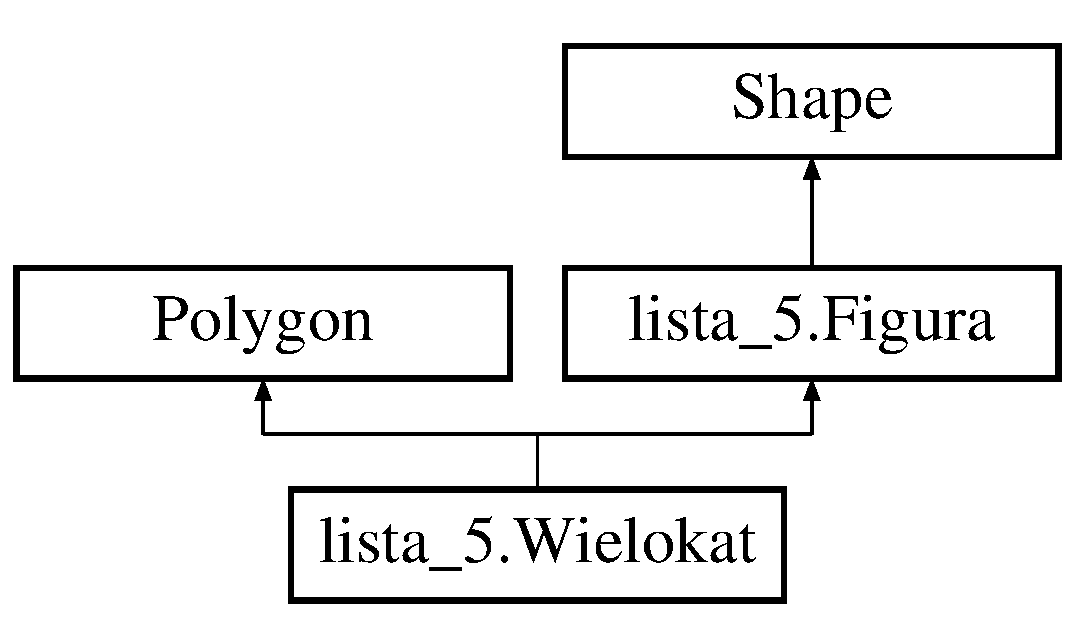
\includegraphics[height=3.000000cm]{classlista__5_1_1_wielokat}
\end{center}
\end{figure}
\subsection*{Public Member Functions}
\begin{DoxyCompactItemize}
\item 
\mbox{\hyperlink{classlista__5_1_1_wielokat_a902f38459eb1935a604537d621f5ca6b}{Wielokat}} (Point d)
\item 
void \mbox{\hyperlink{classlista__5_1_1_wielokat_aca4b29bcec579f442ac566ec3be96d84}{rysuj}} (Point d)
\item 
void \mbox{\hyperlink{classlista__5_1_1_wielokat_a565dc0340d5329d74e5f1f7d0eed1049}{przesun}} (int dx, int dy)
\item 
void \mbox{\hyperlink{classlista__5_1_1_wielokat_ad1df79cd3736bb0fcf3ba2252409f3f8}{wypisz\+Dane}} ()
\item 
String \mbox{\hyperlink{classlista__5_1_1_wielokat_a6391ebe6bc42d42b6bd3041b1a6bd7bd}{zapisz\+Dane}} ()
\item 
void \mbox{\hyperlink{classlista__5_1_1_wielokat_ae863735ff7b742c4703bc142455d34ce}{zmien\+Kolor}} (Graphics2D g2d, Color \mbox{\hyperlink{classlista__5_1_1_wielokat_a6804efa88b78068f50c71ba760dcccc5}{kolor}})
\item 
void \mbox{\hyperlink{classlista__5_1_1_wielokat_a0c33c8213f6796d16aac592f2a961768}{ustaw\+Kolor}} (Graphics2D g2d)
\item 
void \mbox{\hyperlink{classlista__5_1_1_wielokat_a8427c86e5be650cbece5464eee1ac053}{ustaw\+Z\+Odczytu}} (String\mbox{[}$\,$\mbox{]} argumenty)
\item 
void \mbox{\hyperlink{classlista__5_1_1_wielokat_a17cfc98331e2a135886070a4094ac0e6}{zwieksz}} (int zwiekszenie)
\end{DoxyCompactItemize}
\subsection*{Private Member Functions}
\begin{DoxyCompactItemize}
\item 
void \mbox{\hyperlink{classlista__5_1_1_wielokat_ab8e8d6236a7e73b426c6504af3b59f5f}{napraw\+Bounds}} (int xpoints\mbox{[}$\,$\mbox{]}, int ypoints\mbox{[}$\,$\mbox{]}, int npoints)
\item 
Point2\+D.\+Double \mbox{\hyperlink{classlista__5_1_1_wielokat_a8498454fc73a25ba038d48e04bb1e8c0}{srednia\+Point}} (int xpoints\mbox{[}$\,$\mbox{]}, int ypoints\mbox{[}$\,$\mbox{]}, int npoints)
\end{DoxyCompactItemize}
\subsection*{Private Attributes}
\begin{DoxyCompactItemize}
\item 
Color \mbox{\hyperlink{classlista__5_1_1_wielokat_a6804efa88b78068f50c71ba760dcccc5}{kolor}} = Color.\+C\+Y\+AN
\item 
final int \mbox{\hyperlink{classlista__5_1_1_wielokat_a362cfa49edf4875e534bb1f95a59e7af}{min\+\_\+width}} = 70
\item 
final int \mbox{\hyperlink{classlista__5_1_1_wielokat_a0aa7a67f7c10f26e3bf9f4444e5ecb65}{min\+\_\+height}} = 70
\end{DoxyCompactItemize}


\subsection{Detailed Description}
Klasa reprezentująca wielokąt. \begin{DoxySeeAlso}{See also}
\mbox{\hyperlink{interfacelista__5_1_1_figura}{Figura}} 
\end{DoxySeeAlso}


\subsection{Constructor \& Destructor Documentation}
\mbox{\Hypertarget{classlista__5_1_1_wielokat_a902f38459eb1935a604537d621f5ca6b}\label{classlista__5_1_1_wielokat_a902f38459eb1935a604537d621f5ca6b}} 
\index{lista\+\_\+5\+::\+Wielokat@{lista\+\_\+5\+::\+Wielokat}!Wielokat@{Wielokat}}
\index{Wielokat@{Wielokat}!lista\+\_\+5\+::\+Wielokat@{lista\+\_\+5\+::\+Wielokat}}
\subsubsection{\texorpdfstring{Wielokat()}{Wielokat()}}
{\footnotesize\ttfamily lista\+\_\+5.\+Wielokat.\+Wielokat (\begin{DoxyParamCaption}\item[{Point}]{d }\end{DoxyParamCaption})}

Tworzy \mbox{\hyperlink{classlista__5_1_1_wielokat}{Wielokat}}, ustalając współrzędne pierwszego punktu oraz aktualizując prostokąt okalający. 
\begin{DoxyParams}{Parameters}
{\em d} & pierwszy punkt \\
\hline
\end{DoxyParams}


\subsection{Member Function Documentation}
\mbox{\Hypertarget{classlista__5_1_1_wielokat_ab8e8d6236a7e73b426c6504af3b59f5f}\label{classlista__5_1_1_wielokat_ab8e8d6236a7e73b426c6504af3b59f5f}} 
\index{lista\+\_\+5\+::\+Wielokat@{lista\+\_\+5\+::\+Wielokat}!napraw\+Bounds@{napraw\+Bounds}}
\index{napraw\+Bounds@{napraw\+Bounds}!lista\+\_\+5\+::\+Wielokat@{lista\+\_\+5\+::\+Wielokat}}
\subsubsection{\texorpdfstring{napraw\+Bounds()}{naprawBounds()}}
{\footnotesize\ttfamily void lista\+\_\+5.\+Wielokat.\+napraw\+Bounds (\begin{DoxyParamCaption}\item[{int}]{xpoints\mbox{[}$\,$\mbox{]},  }\item[{int}]{ypoints\mbox{[}$\,$\mbox{]},  }\item[{int}]{npoints }\end{DoxyParamCaption})\hspace{0.3cm}{\ttfamily [private]}}

Aktualizuje prostokąt okalający wielokąt. 
\begin{DoxyParams}{Parameters}
{\em xpoints} & tablica wartości odciętych punktów wielokąta\mbox{\hyperlink{}{xpoints}} \\
\hline
{\em ypoints} & tablica wartości rzędnych punktów wielokąta \mbox{\hyperlink{}{ypoints}} \\
\hline
{\em npoints} & liczba punktów wielokąta\mbox{\hyperlink{}{npoints}} \\
\hline
\end{DoxyParams}
\mbox{\Hypertarget{classlista__5_1_1_wielokat_a565dc0340d5329d74e5f1f7d0eed1049}\label{classlista__5_1_1_wielokat_a565dc0340d5329d74e5f1f7d0eed1049}} 
\index{lista\+\_\+5\+::\+Wielokat@{lista\+\_\+5\+::\+Wielokat}!przesun@{przesun}}
\index{przesun@{przesun}!lista\+\_\+5\+::\+Wielokat@{lista\+\_\+5\+::\+Wielokat}}
\subsubsection{\texorpdfstring{przesun()}{przesun()}}
{\footnotesize\ttfamily void lista\+\_\+5.\+Wielokat.\+przesun (\begin{DoxyParamCaption}\item[{int}]{dx,  }\item[{int}]{dy }\end{DoxyParamCaption})}

Zmienia położenie figury. 
\begin{DoxyParams}{Parameters}
{\em dx} & zmiana położenia względem osi x, o którą należy przesunąć figurę \\
\hline
{\em dy} & zmiana położenia względem osi y, o którą należy przesunąć figurę\\
\hline
\end{DoxyParams}
 

Implements \mbox{\hyperlink{interfacelista__5_1_1_figura_a72f085618cf604e8b1632ea733043861}{lista\+\_\+5.\+Figura}}.

\mbox{\Hypertarget{classlista__5_1_1_wielokat_aca4b29bcec579f442ac566ec3be96d84}\label{classlista__5_1_1_wielokat_aca4b29bcec579f442ac566ec3be96d84}} 
\index{lista\+\_\+5\+::\+Wielokat@{lista\+\_\+5\+::\+Wielokat}!rysuj@{rysuj}}
\index{rysuj@{rysuj}!lista\+\_\+5\+::\+Wielokat@{lista\+\_\+5\+::\+Wielokat}}
\subsubsection{\texorpdfstring{rysuj()}{rysuj()}}
{\footnotesize\ttfamily void lista\+\_\+5.\+Wielokat.\+rysuj (\begin{DoxyParamCaption}\item[{Point}]{d }\end{DoxyParamCaption})}

Zmienia właściwości figury podczas jej tworzenia i rysowania; 
\begin{DoxyParams}{Parameters}
{\em d} & nowy
\begin{DoxyCode}
Point 
\end{DoxyCode}
 , który zmienia kształt figury\\
\hline
\end{DoxyParams}
 

Implements \mbox{\hyperlink{interfacelista__5_1_1_figura_a1b238957bac675c57febc970067dfd6d}{lista\+\_\+5.\+Figura}}.

\mbox{\Hypertarget{classlista__5_1_1_wielokat_a8498454fc73a25ba038d48e04bb1e8c0}\label{classlista__5_1_1_wielokat_a8498454fc73a25ba038d48e04bb1e8c0}} 
\index{lista\+\_\+5\+::\+Wielokat@{lista\+\_\+5\+::\+Wielokat}!srednia\+Point@{srednia\+Point}}
\index{srednia\+Point@{srednia\+Point}!lista\+\_\+5\+::\+Wielokat@{lista\+\_\+5\+::\+Wielokat}}
\subsubsection{\texorpdfstring{srednia\+Point()}{sredniaPoint()}}
{\footnotesize\ttfamily Point2\+D.\+Double lista\+\_\+5.\+Wielokat.\+srednia\+Point (\begin{DoxyParamCaption}\item[{int}]{xpoints\mbox{[}$\,$\mbox{]},  }\item[{int}]{ypoints\mbox{[}$\,$\mbox{]},  }\item[{int}]{npoints }\end{DoxyParamCaption})\hspace{0.3cm}{\ttfamily [private]}}

Oblicza środkowy punkt jako średnią arytmetyczną wszystkich punktów. 
\begin{DoxyParams}{Parameters}
{\em xpoints} & tablica wartości odciętych punktów wielokąta\mbox{\hyperlink{}{xpoints}} \\
\hline
{\em ypoints} & tablica wartości rzędnych punktów wielokąta \mbox{\hyperlink{}{ypoints}} \\
\hline
{\em npoints} & liczba punktów wielokąta\mbox{\hyperlink{}{npoints}} \\
\hline
\end{DoxyParams}
\begin{DoxyReturn}{Returns}

\begin{DoxyCode}
Point 
\end{DoxyCode}
 , który traktujemy jako środek przy skalowaniu. 
\end{DoxyReturn}
\mbox{\Hypertarget{classlista__5_1_1_wielokat_a0c33c8213f6796d16aac592f2a961768}\label{classlista__5_1_1_wielokat_a0c33c8213f6796d16aac592f2a961768}} 
\index{lista\+\_\+5\+::\+Wielokat@{lista\+\_\+5\+::\+Wielokat}!ustaw\+Kolor@{ustaw\+Kolor}}
\index{ustaw\+Kolor@{ustaw\+Kolor}!lista\+\_\+5\+::\+Wielokat@{lista\+\_\+5\+::\+Wielokat}}
\subsubsection{\texorpdfstring{ustaw\+Kolor()}{ustawKolor()}}
{\footnotesize\ttfamily void lista\+\_\+5.\+Wielokat.\+ustaw\+Kolor (\begin{DoxyParamCaption}\item[{Graphics2D}]{g2d }\end{DoxyParamCaption})}

Zmienia kolor grafiki na ten, który jest przechowywane w polu kolor. 
\begin{DoxyParams}{Parameters}
{\em g2d} & grafika używana w \mbox{\hyperlink{classlista__5_1_1_wnetrze_aa8676192e150a17230d72de122744a47}{Wnetrze\#paint\+Component}} \\
\hline
\end{DoxyParams}
\begin{DoxySeeAlso}{See also}
\mbox{\hyperlink{interfacelista__5_1_1_figura_aeb0982dc44348dd1fde9266d9d476ed0}{zmien\+Kolor}}
\end{DoxySeeAlso}
 

Implements \mbox{\hyperlink{interfacelista__5_1_1_figura_a3cc13bf7229b288d743be7903b3b61a4}{lista\+\_\+5.\+Figura}}.

\mbox{\Hypertarget{classlista__5_1_1_wielokat_a8427c86e5be650cbece5464eee1ac053}\label{classlista__5_1_1_wielokat_a8427c86e5be650cbece5464eee1ac053}} 
\index{lista\+\_\+5\+::\+Wielokat@{lista\+\_\+5\+::\+Wielokat}!ustaw\+Z\+Odczytu@{ustaw\+Z\+Odczytu}}
\index{ustaw\+Z\+Odczytu@{ustaw\+Z\+Odczytu}!lista\+\_\+5\+::\+Wielokat@{lista\+\_\+5\+::\+Wielokat}}
\subsubsection{\texorpdfstring{ustaw\+Z\+Odczytu()}{ustawZOdczytu()}}
{\footnotesize\ttfamily void lista\+\_\+5.\+Wielokat.\+ustaw\+Z\+Odczytu (\begin{DoxyParamCaption}\item[{String \mbox{[}$\,$\mbox{]}}]{argumenty }\end{DoxyParamCaption})}

Ustawia całą figurę korzystając z danych z pliku. 
\begin{DoxyParams}{Parameters}
{\em argumenty} & tablica danych z odczytu, zawiera informacje determinujące figurę\\
\hline
\end{DoxyParams}
 

Implements \mbox{\hyperlink{interfacelista__5_1_1_figura_a75b72b51014348d839e1f2b81525f264}{lista\+\_\+5.\+Figura}}.

\mbox{\Hypertarget{classlista__5_1_1_wielokat_ad1df79cd3736bb0fcf3ba2252409f3f8}\label{classlista__5_1_1_wielokat_ad1df79cd3736bb0fcf3ba2252409f3f8}} 
\index{lista\+\_\+5\+::\+Wielokat@{lista\+\_\+5\+::\+Wielokat}!wypisz\+Dane@{wypisz\+Dane}}
\index{wypisz\+Dane@{wypisz\+Dane}!lista\+\_\+5\+::\+Wielokat@{lista\+\_\+5\+::\+Wielokat}}
\subsubsection{\texorpdfstring{wypisz\+Dane()}{wypiszDane()}}
{\footnotesize\ttfamily void lista\+\_\+5.\+Wielokat.\+wypisz\+Dane (\begin{DoxyParamCaption}{ }\end{DoxyParamCaption})}

Wypisuje dane związane z figurą w \mbox{\hyperlink{classlista__5_1_1_stopka_a8e8ef21758defd5b137e609b00d2f59e}{Stopka\#dane}} 

Implements \mbox{\hyperlink{interfacelista__5_1_1_figura_aaddd90c61fd1632655cb031efafe1a7d}{lista\+\_\+5.\+Figura}}.

\mbox{\Hypertarget{classlista__5_1_1_wielokat_a6391ebe6bc42d42b6bd3041b1a6bd7bd}\label{classlista__5_1_1_wielokat_a6391ebe6bc42d42b6bd3041b1a6bd7bd}} 
\index{lista\+\_\+5\+::\+Wielokat@{lista\+\_\+5\+::\+Wielokat}!zapisz\+Dane@{zapisz\+Dane}}
\index{zapisz\+Dane@{zapisz\+Dane}!lista\+\_\+5\+::\+Wielokat@{lista\+\_\+5\+::\+Wielokat}}
\subsubsection{\texorpdfstring{zapisz\+Dane()}{zapiszDane()}}
{\footnotesize\ttfamily String lista\+\_\+5.\+Wielokat.\+zapisz\+Dane (\begin{DoxyParamCaption}{ }\end{DoxyParamCaption})}

Przygotowuje informacje o figurze do zapisania. \begin{DoxyReturn}{Returns}
linia, która zostanie zapisana w pliku
\end{DoxyReturn}
 

Implements \mbox{\hyperlink{interfacelista__5_1_1_figura_a9d60d64b495755a3e48a3eee549a728d}{lista\+\_\+5.\+Figura}}.

\mbox{\Hypertarget{classlista__5_1_1_wielokat_ae863735ff7b742c4703bc142455d34ce}\label{classlista__5_1_1_wielokat_ae863735ff7b742c4703bc142455d34ce}} 
\index{lista\+\_\+5\+::\+Wielokat@{lista\+\_\+5\+::\+Wielokat}!zmien\+Kolor@{zmien\+Kolor}}
\index{zmien\+Kolor@{zmien\+Kolor}!lista\+\_\+5\+::\+Wielokat@{lista\+\_\+5\+::\+Wielokat}}
\subsubsection{\texorpdfstring{zmien\+Kolor()}{zmienKolor()}}
{\footnotesize\ttfamily void lista\+\_\+5.\+Wielokat.\+zmien\+Kolor (\begin{DoxyParamCaption}\item[{Graphics2D}]{g2d,  }\item[{Color}]{kolor }\end{DoxyParamCaption})}

Aktualizuje pole kolor obecne w każdej figurze. 
\begin{DoxyParams}{Parameters}
{\em g2d} & grafika używana w \mbox{\hyperlink{classlista__5_1_1_wnetrze_aa8676192e150a17230d72de122744a47}{Wnetrze\#paint\+Component}} \\
\hline
{\em kolor} & pożądany kolor \\
\hline
\end{DoxyParams}
\begin{DoxySeeAlso}{See also}
\mbox{\hyperlink{interfacelista__5_1_1_figura_a3cc13bf7229b288d743be7903b3b61a4}{ustaw\+Kolor}}
\end{DoxySeeAlso}
 

Implements \mbox{\hyperlink{interfacelista__5_1_1_figura_aeb0982dc44348dd1fde9266d9d476ed0}{lista\+\_\+5.\+Figura}}.

\mbox{\Hypertarget{classlista__5_1_1_wielokat_a17cfc98331e2a135886070a4094ac0e6}\label{classlista__5_1_1_wielokat_a17cfc98331e2a135886070a4094ac0e6}} 
\index{lista\+\_\+5\+::\+Wielokat@{lista\+\_\+5\+::\+Wielokat}!zwieksz@{zwieksz}}
\index{zwieksz@{zwieksz}!lista\+\_\+5\+::\+Wielokat@{lista\+\_\+5\+::\+Wielokat}}
\subsubsection{\texorpdfstring{zwieksz()}{zwieksz()}}
{\footnotesize\ttfamily void lista\+\_\+5.\+Wielokat.\+zwieksz (\begin{DoxyParamCaption}\item[{int}]{zwiekszenie }\end{DoxyParamCaption})}

Powiększa rozmiary figury. 
\begin{DoxyParams}{Parameters}
{\em zwiekszenie} & wartość, o którą należy zwiększyć figurę przy skalowaniu\\
\hline
\end{DoxyParams}
, pamiętając o wartościach minimalnych. \begin{DoxySeeAlso}{See also}
\mbox{\hyperlink{classlista__5_1_1_wielokat_a362cfa49edf4875e534bb1f95a59e7af}{min\+\_\+width}} 

\mbox{\hyperlink{classlista__5_1_1_wielokat_a0aa7a67f7c10f26e3bf9f4444e5ecb65}{min\+\_\+height}} 
\end{DoxySeeAlso}


Implements \mbox{\hyperlink{interfacelista__5_1_1_figura_a6813d7ac31e5118bcb34b9b29868ce5f}{lista\+\_\+5.\+Figura}}.



\subsection{Member Data Documentation}
\mbox{\Hypertarget{classlista__5_1_1_wielokat_a6804efa88b78068f50c71ba760dcccc5}\label{classlista__5_1_1_wielokat_a6804efa88b78068f50c71ba760dcccc5}} 
\index{lista\+\_\+5\+::\+Wielokat@{lista\+\_\+5\+::\+Wielokat}!kolor@{kolor}}
\index{kolor@{kolor}!lista\+\_\+5\+::\+Wielokat@{lista\+\_\+5\+::\+Wielokat}}
\subsubsection{\texorpdfstring{kolor}{kolor}}
{\footnotesize\ttfamily Color lista\+\_\+5.\+Wielokat.\+kolor = Color.\+C\+Y\+AN\hspace{0.3cm}{\ttfamily [private]}}


\begin{DoxyCode}
Color 
\end{DoxyCode}
 , domyślnie ustawiony na
\begin{DoxyCode}
Color.ORANGE 
\end{DoxyCode}
 \mbox{\Hypertarget{classlista__5_1_1_wielokat_a0aa7a67f7c10f26e3bf9f4444e5ecb65}\label{classlista__5_1_1_wielokat_a0aa7a67f7c10f26e3bf9f4444e5ecb65}} 
\index{lista\+\_\+5\+::\+Wielokat@{lista\+\_\+5\+::\+Wielokat}!min\+\_\+height@{min\+\_\+height}}
\index{min\+\_\+height@{min\+\_\+height}!lista\+\_\+5\+::\+Wielokat@{lista\+\_\+5\+::\+Wielokat}}
\subsubsection{\texorpdfstring{min\+\_\+height}{min\_height}}
{\footnotesize\ttfamily final int lista\+\_\+5.\+Wielokat.\+min\+\_\+height = 70\hspace{0.3cm}{\ttfamily [private]}}

Minimalna wysokość, która jest nieprzekraczalna przy zmniejszaniu. \mbox{\Hypertarget{classlista__5_1_1_wielokat_a362cfa49edf4875e534bb1f95a59e7af}\label{classlista__5_1_1_wielokat_a362cfa49edf4875e534bb1f95a59e7af}} 
\index{lista\+\_\+5\+::\+Wielokat@{lista\+\_\+5\+::\+Wielokat}!min\+\_\+width@{min\+\_\+width}}
\index{min\+\_\+width@{min\+\_\+width}!lista\+\_\+5\+::\+Wielokat@{lista\+\_\+5\+::\+Wielokat}}
\subsubsection{\texorpdfstring{min\+\_\+width}{min\_width}}
{\footnotesize\ttfamily final int lista\+\_\+5.\+Wielokat.\+min\+\_\+width = 70\hspace{0.3cm}{\ttfamily [private]}}

Minimalna szerokość, która jest nieprzekraczalna przy zmniejszaniu. 

The documentation for this class was generated from the following file\+:\begin{DoxyCompactItemize}
\item 
lista\+\_\+5/\mbox{\hyperlink{_wielokat_8java}{Wielokat.\+java}}\end{DoxyCompactItemize}

\hypertarget{classlista__5_1_1_wnetrze}{}\section{lista\+\_\+5.\+Wnetrze Class Reference}
\label{classlista__5_1_1_wnetrze}\index{lista\+\_\+5.\+Wnetrze@{lista\+\_\+5.\+Wnetrze}}
Inheritance diagram for lista\+\_\+5.\+Wnetrze\+:\begin{figure}[H]
\begin{center}
\leavevmode
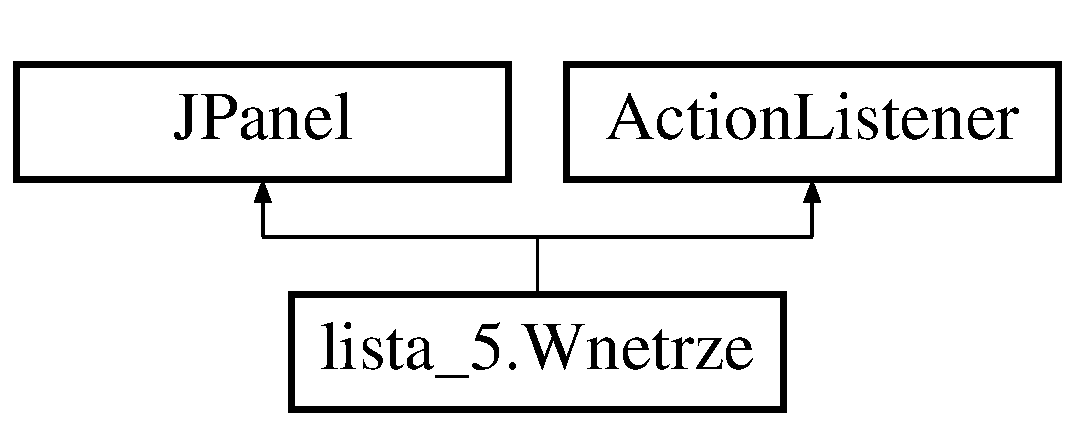
\includegraphics[height=2.000000cm]{classlista__5_1_1_wnetrze}
\end{center}
\end{figure}
\subsection*{Classes}
\begin{DoxyCompactItemize}
\item 
class \mbox{\hyperlink{classlista__5_1_1_wnetrze_1_1_moj_mouse_adapter}{Moj\+Mouse\+Adapter}}
\end{DoxyCompactItemize}
\subsection*{Public Member Functions}
\begin{DoxyCompactItemize}
\item 
\mbox{\hyperlink{classlista__5_1_1_wnetrze_a7fc5065e5b578f1613050a099df86864}{Wnetrze}} ()
\item 
void \mbox{\hyperlink{classlista__5_1_1_wnetrze_aa5e96d1ba61b233b93c6d8a71931be07}{usun\+Wielokat}} ()
\item 
void \mbox{\hyperlink{classlista__5_1_1_wnetrze_aa8676192e150a17230d72de122744a47}{paint\+Component}} (Graphics g)
\item 
void \mbox{\hyperlink{classlista__5_1_1_wnetrze_a2f9c15a3d95e323370ae52a28881d73f}{action\+Performed}} (Action\+Event e)
\item 
void \mbox{\hyperlink{classlista__5_1_1_wnetrze_a3f2f50d048d7c41f2cbbb7f91f59c077}{zapisz}} ()  throws I\+O\+Exception      
\item 
void \mbox{\hyperlink{classlista__5_1_1_wnetrze_ad5ebd5c04f2c4b9de6954303c96a5856}{odczyt}} ()  throws I\+O\+Exception     
\end{DoxyCompactItemize}
\subsection*{Public Attributes}
\begin{DoxyCompactItemize}
\item 
boolean \mbox{\hyperlink{classlista__5_1_1_wnetrze_aafcbd167c4a739f34f4c8420f41e7290}{czy\+Wielokat}} = false
\end{DoxyCompactItemize}
\subsection*{Private Attributes}
\begin{DoxyCompactItemize}
\item 
Array\+List$<$ \mbox{\hyperlink{interfacelista__5_1_1_figura}{Figura}} $>$ \mbox{\hyperlink{classlista__5_1_1_wnetrze_abeebc1924e88a0d99f63f06989b26de6}{figury}}
\item 
\mbox{\hyperlink{interfacelista__5_1_1_figura}{Figura}} \mbox{\hyperlink{classlista__5_1_1_wnetrze_a9ca273969f43e95e7cbb14771b661832}{figura\+Menu}}
\item 
\mbox{\hyperlink{classlista__5_1_1_wielokat}{Wielokat}} \mbox{\hyperlink{classlista__5_1_1_wnetrze_a6f5256e1e24b7cc70ea083655a3e649b}{wielokat\+Rys}}
\item 
\mbox{\hyperlink{classlista__5_1_1_menu_kontekstowe}{Menu\+Kontekstowe}} \mbox{\hyperlink{classlista__5_1_1_wnetrze_a3b82cd912cfe874fd313ffc40687ddf6}{menu}}
\item 
Graphics2D \mbox{\hyperlink{classlista__5_1_1_wnetrze_a7aa207b33c99ffe3b8f8e4a2f7e22632}{g2d}}
\end{DoxyCompactItemize}


\subsection{Detailed Description}
Najważniejsza klasa w programie -\/ zajmuje się rysowaniem i wszystkimi akcjami związanymi z działalnością użytkownika w obrębie rysowania. Jest to panel znajdujący się w centrum programu. Ma w sobie jedną klasę wewnętrzną \mbox{\hyperlink{classlista__5_1_1_wnetrze_1_1_moj_mouse_adapter}{Moj\+Mouse\+Adapter}}.

\begin{DoxySeeAlso}{See also}
Action\+Listener 
\end{DoxySeeAlso}


\subsection{Constructor \& Destructor Documentation}
\mbox{\Hypertarget{classlista__5_1_1_wnetrze_a7fc5065e5b578f1613050a099df86864}\label{classlista__5_1_1_wnetrze_a7fc5065e5b578f1613050a099df86864}} 
\index{lista\+\_\+5\+::\+Wnetrze@{lista\+\_\+5\+::\+Wnetrze}!Wnetrze@{Wnetrze}}
\index{Wnetrze@{Wnetrze}!lista\+\_\+5\+::\+Wnetrze@{lista\+\_\+5\+::\+Wnetrze}}
\subsubsection{\texorpdfstring{Wnetrze()}{Wnetrze()}}
{\footnotesize\ttfamily lista\+\_\+5.\+Wnetrze.\+Wnetrze (\begin{DoxyParamCaption}{ }\end{DoxyParamCaption})}

Powołuje do życia obiekty i dodaje
\begin{DoxyCode}
MojMouseAdapter 
\end{DoxyCode}
 . 

\subsection{Member Function Documentation}
\mbox{\Hypertarget{classlista__5_1_1_wnetrze_a2f9c15a3d95e323370ae52a28881d73f}\label{classlista__5_1_1_wnetrze_a2f9c15a3d95e323370ae52a28881d73f}} 
\index{lista\+\_\+5\+::\+Wnetrze@{lista\+\_\+5\+::\+Wnetrze}!action\+Performed@{action\+Performed}}
\index{action\+Performed@{action\+Performed}!lista\+\_\+5\+::\+Wnetrze@{lista\+\_\+5\+::\+Wnetrze}}
\subsubsection{\texorpdfstring{action\+Performed()}{actionPerformed()}}
{\footnotesize\ttfamily void lista\+\_\+5.\+Wnetrze.\+action\+Performed (\begin{DoxyParamCaption}\item[{Action\+Event}]{e }\end{DoxyParamCaption})}

Zmienia kolor figury. \mbox{\Hypertarget{classlista__5_1_1_wnetrze_ad5ebd5c04f2c4b9de6954303c96a5856}\label{classlista__5_1_1_wnetrze_ad5ebd5c04f2c4b9de6954303c96a5856}} 
\index{lista\+\_\+5\+::\+Wnetrze@{lista\+\_\+5\+::\+Wnetrze}!odczyt@{odczyt}}
\index{odczyt@{odczyt}!lista\+\_\+5\+::\+Wnetrze@{lista\+\_\+5\+::\+Wnetrze}}
\subsubsection{\texorpdfstring{odczyt()}{odczyt()}}
{\footnotesize\ttfamily void lista\+\_\+5.\+Wnetrze.\+odczyt (\begin{DoxyParamCaption}{ }\end{DoxyParamCaption}) throws I\+O\+Exception}

Najpierw czyści panel, a następnie odczytuje stan figur z pliku tekstowego. 
\begin{DoxyExceptions}{Exceptions}
{\em I\+O\+Exception} & wyjątek, mogący wystąpić przy braku możliwości odczytu z pliku \\
\hline
\end{DoxyExceptions}
\mbox{\Hypertarget{classlista__5_1_1_wnetrze_aa8676192e150a17230d72de122744a47}\label{classlista__5_1_1_wnetrze_aa8676192e150a17230d72de122744a47}} 
\index{lista\+\_\+5\+::\+Wnetrze@{lista\+\_\+5\+::\+Wnetrze}!paint\+Component@{paint\+Component}}
\index{paint\+Component@{paint\+Component}!lista\+\_\+5\+::\+Wnetrze@{lista\+\_\+5\+::\+Wnetrze}}
\subsubsection{\texorpdfstring{paint\+Component()}{paintComponent()}}
{\footnotesize\ttfamily void lista\+\_\+5.\+Wnetrze.\+paint\+Component (\begin{DoxyParamCaption}\item[{Graphics}]{g }\end{DoxyParamCaption})}

Metoda odpowiadająca za rysowanie, rysuje po kolei wszystkie figury znajdujące się w \mbox{\hyperlink{classlista__5_1_1_wnetrze_abeebc1924e88a0d99f63f06989b26de6}{figury}}. Jeśli wielokąt jest w trakcie rysowania, to rysuje jedynie kształt, po zakończeniu wypełnia go. \mbox{\Hypertarget{classlista__5_1_1_wnetrze_aa5e96d1ba61b233b93c6d8a71931be07}\label{classlista__5_1_1_wnetrze_aa5e96d1ba61b233b93c6d8a71931be07}} 
\index{lista\+\_\+5\+::\+Wnetrze@{lista\+\_\+5\+::\+Wnetrze}!usun\+Wielokat@{usun\+Wielokat}}
\index{usun\+Wielokat@{usun\+Wielokat}!lista\+\_\+5\+::\+Wnetrze@{lista\+\_\+5\+::\+Wnetrze}}
\subsubsection{\texorpdfstring{usun\+Wielokat()}{usunWielokat()}}
{\footnotesize\ttfamily void lista\+\_\+5.\+Wnetrze.\+usun\+Wielokat (\begin{DoxyParamCaption}{ }\end{DoxyParamCaption})}

Usuwa wielokąt z \mbox{\hyperlink{classlista__5_1_1_wnetrze_abeebc1924e88a0d99f63f06989b26de6}{figury}} i z ekranu. \mbox{\Hypertarget{classlista__5_1_1_wnetrze_a3f2f50d048d7c41f2cbbb7f91f59c077}\label{classlista__5_1_1_wnetrze_a3f2f50d048d7c41f2cbbb7f91f59c077}} 
\index{lista\+\_\+5\+::\+Wnetrze@{lista\+\_\+5\+::\+Wnetrze}!zapisz@{zapisz}}
\index{zapisz@{zapisz}!lista\+\_\+5\+::\+Wnetrze@{lista\+\_\+5\+::\+Wnetrze}}
\subsubsection{\texorpdfstring{zapisz()}{zapisz()}}
{\footnotesize\ttfamily void lista\+\_\+5.\+Wnetrze.\+zapisz (\begin{DoxyParamCaption}{ }\end{DoxyParamCaption}) throws I\+O\+Exception}

Zapisuje obecny stan figur do pliku tekstowego. 
\begin{DoxyExceptions}{Exceptions}
{\em I\+O\+Exception} & wyjątek, mogący wystąpić przy braku możliwości zapisu do pliku \\
\hline
\end{DoxyExceptions}


\subsection{Member Data Documentation}
\mbox{\Hypertarget{classlista__5_1_1_wnetrze_aafcbd167c4a739f34f4c8420f41e7290}\label{classlista__5_1_1_wnetrze_aafcbd167c4a739f34f4c8420f41e7290}} 
\index{lista\+\_\+5\+::\+Wnetrze@{lista\+\_\+5\+::\+Wnetrze}!czy\+Wielokat@{czy\+Wielokat}}
\index{czy\+Wielokat@{czy\+Wielokat}!lista\+\_\+5\+::\+Wnetrze@{lista\+\_\+5\+::\+Wnetrze}}
\subsubsection{\texorpdfstring{czy\+Wielokat}{czyWielokat}}
{\footnotesize\ttfamily boolean lista\+\_\+5.\+Wnetrze.\+czy\+Wielokat = false}


\begin{DoxyCode}
\textcolor{keyword}{true} 
\end{DoxyCode}
 -\/ jeśli jakiś wielokąt jest obecnie rysowany,
\begin{DoxyCode}
\textcolor{keyword}{false} 
\end{DoxyCode}
 -\/ jeśli żaden wielokąt nie jest obecnie rysowany \mbox{\Hypertarget{classlista__5_1_1_wnetrze_a9ca273969f43e95e7cbb14771b661832}\label{classlista__5_1_1_wnetrze_a9ca273969f43e95e7cbb14771b661832}} 
\index{lista\+\_\+5\+::\+Wnetrze@{lista\+\_\+5\+::\+Wnetrze}!figura\+Menu@{figura\+Menu}}
\index{figura\+Menu@{figura\+Menu}!lista\+\_\+5\+::\+Wnetrze@{lista\+\_\+5\+::\+Wnetrze}}
\subsubsection{\texorpdfstring{figura\+Menu}{figuraMenu}}
{\footnotesize\ttfamily \mbox{\hyperlink{interfacelista__5_1_1_figura}{Figura}} lista\+\_\+5.\+Wnetrze.\+figura\+Menu\hspace{0.3cm}{\ttfamily [private]}}

\mbox{\hyperlink{interfacelista__5_1_1_figura}{Figura}}, na rzecz której wywołano menu z kolorami. \mbox{\Hypertarget{classlista__5_1_1_wnetrze_abeebc1924e88a0d99f63f06989b26de6}\label{classlista__5_1_1_wnetrze_abeebc1924e88a0d99f63f06989b26de6}} 
\index{lista\+\_\+5\+::\+Wnetrze@{lista\+\_\+5\+::\+Wnetrze}!figury@{figury}}
\index{figury@{figury}!lista\+\_\+5\+::\+Wnetrze@{lista\+\_\+5\+::\+Wnetrze}}
\subsubsection{\texorpdfstring{figury}{figury}}
{\footnotesize\ttfamily Array\+List$<$\mbox{\hyperlink{interfacelista__5_1_1_figura}{Figura}}$>$ lista\+\_\+5.\+Wnetrze.\+figury\hspace{0.3cm}{\ttfamily [private]}}

Array\+List, która ma w sobie wszystkie powstałe figury. \begin{DoxySeeAlso}{See also}
\mbox{\hyperlink{interfacelista__5_1_1_figura}{Figura}} 
\end{DoxySeeAlso}
\mbox{\Hypertarget{classlista__5_1_1_wnetrze_a7aa207b33c99ffe3b8f8e4a2f7e22632}\label{classlista__5_1_1_wnetrze_a7aa207b33c99ffe3b8f8e4a2f7e22632}} 
\index{lista\+\_\+5\+::\+Wnetrze@{lista\+\_\+5\+::\+Wnetrze}!g2d@{g2d}}
\index{g2d@{g2d}!lista\+\_\+5\+::\+Wnetrze@{lista\+\_\+5\+::\+Wnetrze}}
\subsubsection{\texorpdfstring{g2d}{g2d}}
{\footnotesize\ttfamily Graphics2D lista\+\_\+5.\+Wnetrze.\+g2d\hspace{0.3cm}{\ttfamily [private]}}

Główny obiekt klasy
\begin{DoxyCode}
Graphics2D 
\end{DoxyCode}
 , pozwalający nam na rysowanie. \mbox{\Hypertarget{classlista__5_1_1_wnetrze_a3b82cd912cfe874fd313ffc40687ddf6}\label{classlista__5_1_1_wnetrze_a3b82cd912cfe874fd313ffc40687ddf6}} 
\index{lista\+\_\+5\+::\+Wnetrze@{lista\+\_\+5\+::\+Wnetrze}!menu@{menu}}
\index{menu@{menu}!lista\+\_\+5\+::\+Wnetrze@{lista\+\_\+5\+::\+Wnetrze}}
\subsubsection{\texorpdfstring{menu}{menu}}
{\footnotesize\ttfamily \mbox{\hyperlink{classlista__5_1_1_menu_kontekstowe}{Menu\+Kontekstowe}} lista\+\_\+5.\+Wnetrze.\+menu\hspace{0.3cm}{\ttfamily [private]}}

Menu pozwalające na zmianę kolorów. \mbox{\Hypertarget{classlista__5_1_1_wnetrze_a6f5256e1e24b7cc70ea083655a3e649b}\label{classlista__5_1_1_wnetrze_a6f5256e1e24b7cc70ea083655a3e649b}} 
\index{lista\+\_\+5\+::\+Wnetrze@{lista\+\_\+5\+::\+Wnetrze}!wielokat\+Rys@{wielokat\+Rys}}
\index{wielokat\+Rys@{wielokat\+Rys}!lista\+\_\+5\+::\+Wnetrze@{lista\+\_\+5\+::\+Wnetrze}}
\subsubsection{\texorpdfstring{wielokat\+Rys}{wielokatRys}}
{\footnotesize\ttfamily \mbox{\hyperlink{classlista__5_1_1_wielokat}{Wielokat}} lista\+\_\+5.\+Wnetrze.\+wielokat\+Rys\hspace{0.3cm}{\ttfamily [private]}}

Obecnie rysowany wielokąt. 

The documentation for this class was generated from the following file\+:\begin{DoxyCompactItemize}
\item 
lista\+\_\+5/\mbox{\hyperlink{_wnetrze_8java}{Wnetrze.\+java}}\end{DoxyCompactItemize}

\hypertarget{classlista__5_1_1_wyglad}{}\section{lista\+\_\+5.\+Wyglad Class Reference}
\label{classlista__5_1_1_wyglad}\index{lista\+\_\+5.\+Wyglad@{lista\+\_\+5.\+Wyglad}}
Inheritance diagram for lista\+\_\+5.\+Wyglad\+:\begin{figure}[H]
\begin{center}
\leavevmode
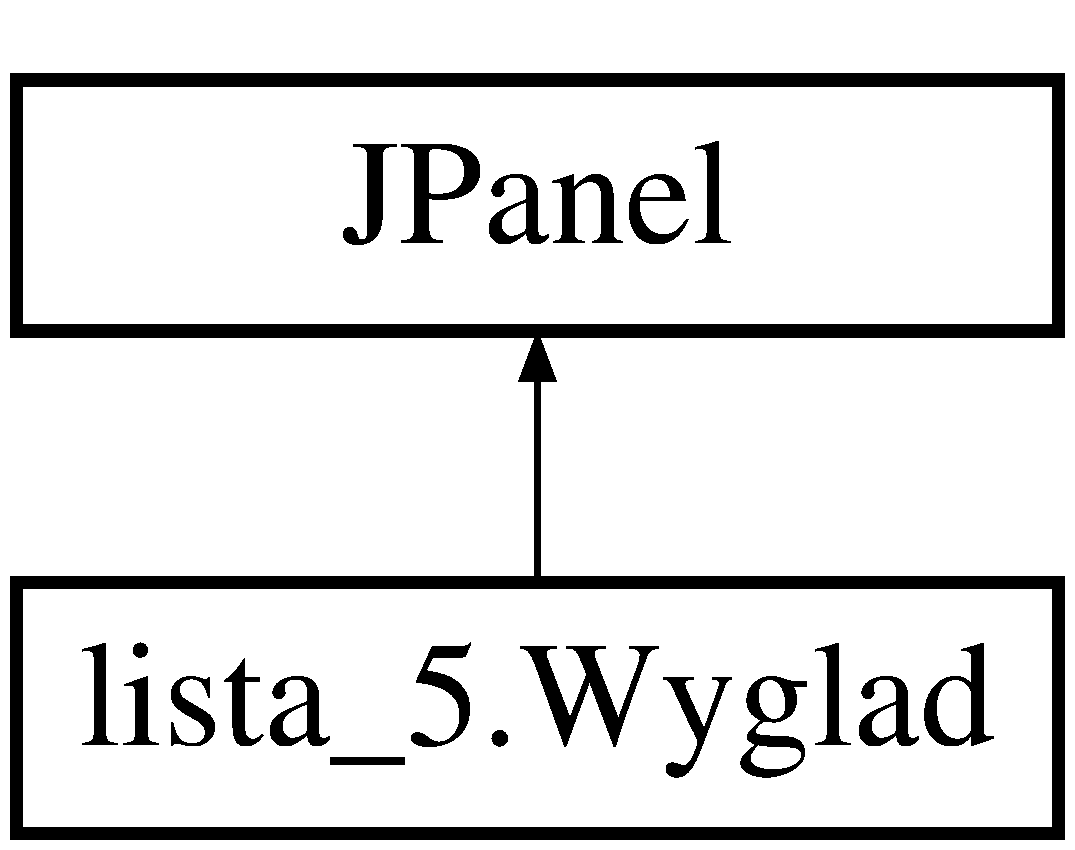
\includegraphics[height=2.000000cm]{classlista__5_1_1_wyglad}
\end{center}
\end{figure}
\subsection*{Public Member Functions}
\begin{DoxyCompactItemize}
\item 
\mbox{\hyperlink{classlista__5_1_1_wyglad_aa8dcaceecff0bce220abc4e796ff44d5}{Wyglad}} ()
\end{DoxyCompactItemize}
\subsection*{Package Attributes}
\begin{DoxyCompactItemize}
\item 
\mbox{\hyperlink{classlista__5_1_1_stopka}{Stopka}} \mbox{\hyperlink{classlista__5_1_1_wyglad_a73653db64a554970f69f0074013c2efd}{stopka}}
\item 
\mbox{\hyperlink{classlista__5_1_1_prawy_bok}{Prawy\+Bok}} \mbox{\hyperlink{classlista__5_1_1_wyglad_aa59e5268c008769e2b033eea9441caff}{prawy\+Bok}}
\item 
\mbox{\hyperlink{classlista__5_1_1_wnetrze}{Wnetrze}} \mbox{\hyperlink{classlista__5_1_1_wyglad_a76f7663502062e7784d87c1cc855721b}{wnetrze}}
\end{DoxyCompactItemize}


\subsection{Detailed Description}
Klasa, ktorej obiekt jest panelem calkowicie wypelniajacym okno. \begin{DoxySeeAlso}{See also}
Paint 
\end{DoxySeeAlso}


\subsection{Constructor \& Destructor Documentation}
\mbox{\Hypertarget{classlista__5_1_1_wyglad_aa8dcaceecff0bce220abc4e796ff44d5}\label{classlista__5_1_1_wyglad_aa8dcaceecff0bce220abc4e796ff44d5}} 
\index{lista\+\_\+5\+::\+Wyglad@{lista\+\_\+5\+::\+Wyglad}!Wyglad@{Wyglad}}
\index{Wyglad@{Wyglad}!lista\+\_\+5\+::\+Wyglad@{lista\+\_\+5\+::\+Wyglad}}
\subsubsection{\texorpdfstring{Wyglad()}{Wyglad()}}
{\footnotesize\ttfamily lista\+\_\+5.\+Wyglad.\+Wyglad (\begin{DoxyParamCaption}{ }\end{DoxyParamCaption})}



\subsection{Member Data Documentation}
\mbox{\Hypertarget{classlista__5_1_1_wyglad_aa59e5268c008769e2b033eea9441caff}\label{classlista__5_1_1_wyglad_aa59e5268c008769e2b033eea9441caff}} 
\index{lista\+\_\+5\+::\+Wyglad@{lista\+\_\+5\+::\+Wyglad}!prawy\+Bok@{prawy\+Bok}}
\index{prawy\+Bok@{prawy\+Bok}!lista\+\_\+5\+::\+Wyglad@{lista\+\_\+5\+::\+Wyglad}}
\subsubsection{\texorpdfstring{prawy\+Bok}{prawyBok}}
{\footnotesize\ttfamily \mbox{\hyperlink{classlista__5_1_1_prawy_bok}{Prawy\+Bok}} lista\+\_\+5.\+Wyglad.\+prawy\+Bok\hspace{0.3cm}{\ttfamily [package]}}

\mbox{\Hypertarget{classlista__5_1_1_wyglad_a73653db64a554970f69f0074013c2efd}\label{classlista__5_1_1_wyglad_a73653db64a554970f69f0074013c2efd}} 
\index{lista\+\_\+5\+::\+Wyglad@{lista\+\_\+5\+::\+Wyglad}!stopka@{stopka}}
\index{stopka@{stopka}!lista\+\_\+5\+::\+Wyglad@{lista\+\_\+5\+::\+Wyglad}}
\subsubsection{\texorpdfstring{stopka}{stopka}}
{\footnotesize\ttfamily \mbox{\hyperlink{classlista__5_1_1_stopka}{Stopka}} lista\+\_\+5.\+Wyglad.\+stopka\hspace{0.3cm}{\ttfamily [package]}}

\mbox{\Hypertarget{classlista__5_1_1_wyglad_a76f7663502062e7784d87c1cc855721b}\label{classlista__5_1_1_wyglad_a76f7663502062e7784d87c1cc855721b}} 
\index{lista\+\_\+5\+::\+Wyglad@{lista\+\_\+5\+::\+Wyglad}!wnetrze@{wnetrze}}
\index{wnetrze@{wnetrze}!lista\+\_\+5\+::\+Wyglad@{lista\+\_\+5\+::\+Wyglad}}
\subsubsection{\texorpdfstring{wnetrze}{wnetrze}}
{\footnotesize\ttfamily \mbox{\hyperlink{classlista__5_1_1_wnetrze}{Wnetrze}} lista\+\_\+5.\+Wyglad.\+wnetrze\hspace{0.3cm}{\ttfamily [package]}}



The documentation for this class was generated from the following file\+:\begin{DoxyCompactItemize}
\item 
lista\+\_\+5/\mbox{\hyperlink{_painty_8java}{Painty.\+java}}\end{DoxyCompactItemize}

\chapter{File Documentation}
\hypertarget{_figura_8java}{}\section{lista\+\_\+5/\+Figura.java File Reference}
\label{_figura_8java}\index{lista\+\_\+5/\+Figura.\+java@{lista\+\_\+5/\+Figura.\+java}}
\subsection*{Classes}
\begin{DoxyCompactItemize}
\item 
interface \mbox{\hyperlink{interfacelista__5_1_1_figura}{lista\+\_\+5.\+Figura}}
\end{DoxyCompactItemize}
\subsection*{Packages}
\begin{DoxyCompactItemize}
\item 
package \mbox{\hyperlink{namespacelista__5}{lista\+\_\+5}}
\end{DoxyCompactItemize}

\hypertarget{_info_8java}{}\section{lista\+\_\+5/\+Info.java File Reference}
\label{_info_8java}\index{lista\+\_\+5/\+Info.\+java@{lista\+\_\+5/\+Info.\+java}}
\subsection*{Classes}
\begin{DoxyCompactItemize}
\item 
class \mbox{\hyperlink{classlista__5_1_1_info}{lista\+\_\+5.\+Info}}
\end{DoxyCompactItemize}
\subsection*{Packages}
\begin{DoxyCompactItemize}
\item 
package \mbox{\hyperlink{namespacelista__5}{lista\+\_\+5}}
\end{DoxyCompactItemize}

\hypertarget{_kolo_8java}{}\section{lista\+\_\+5/\+Kolo.java File Reference}
\label{_kolo_8java}\index{lista\+\_\+5/\+Kolo.\+java@{lista\+\_\+5/\+Kolo.\+java}}
\subsection*{Classes}
\begin{DoxyCompactItemize}
\item 
class \mbox{\hyperlink{classlista__5_1_1_kolo}{lista\+\_\+5.\+Kolo}}
\end{DoxyCompactItemize}
\subsection*{Packages}
\begin{DoxyCompactItemize}
\item 
package \mbox{\hyperlink{namespacelista__5}{lista\+\_\+5}}
\end{DoxyCompactItemize}

\hypertarget{_menu_kontekstowe_8java}{}\section{lista\+\_\+5/\+Menu\+Kontekstowe.java File Reference}
\label{_menu_kontekstowe_8java}\index{lista\+\_\+5/\+Menu\+Kontekstowe.\+java@{lista\+\_\+5/\+Menu\+Kontekstowe.\+java}}
\subsection*{Classes}
\begin{DoxyCompactItemize}
\item 
class \mbox{\hyperlink{classlista__5_1_1_menu_kontekstowe}{lista\+\_\+5.\+Menu\+Kontekstowe}}
\end{DoxyCompactItemize}
\subsection*{Packages}
\begin{DoxyCompactItemize}
\item 
package \mbox{\hyperlink{namespacelista__5}{lista\+\_\+5}}
\end{DoxyCompactItemize}

\hypertarget{_painty_8java}{}\section{lista\+\_\+5/\+Painty.java File Reference}
\label{_painty_8java}\index{lista\+\_\+5/\+Painty.\+java@{lista\+\_\+5/\+Painty.\+java}}
\subsection*{Classes}
\begin{DoxyCompactItemize}
\item 
class \mbox{\hyperlink{classlista__5_1_1_wyglad}{lista\+\_\+5.\+Wyglad}}
\item 
class \mbox{\hyperlink{classlista__5_1_1_painty}{lista\+\_\+5.\+Painty}}
\end{DoxyCompactItemize}
\subsection*{Packages}
\begin{DoxyCompactItemize}
\item 
package \mbox{\hyperlink{namespacelista__5}{lista\+\_\+5}}
\end{DoxyCompactItemize}

\hypertarget{_prawy_bok_8java}{}\section{lista\+\_\+5/\+Prawy\+Bok.java File Reference}
\label{_prawy_bok_8java}\index{lista\+\_\+5/\+Prawy\+Bok.\+java@{lista\+\_\+5/\+Prawy\+Bok.\+java}}
\subsection*{Classes}
\begin{DoxyCompactItemize}
\item 
class \mbox{\hyperlink{classlista__5_1_1_prawy_bok}{lista\+\_\+5.\+Prawy\+Bok}}
\end{DoxyCompactItemize}
\subsection*{Packages}
\begin{DoxyCompactItemize}
\item 
package \mbox{\hyperlink{namespacelista__5}{lista\+\_\+5}}
\end{DoxyCompactItemize}

\hypertarget{_prostokat_8java}{}\section{lista\+\_\+5/\+Prostokat.java File Reference}
\label{_prostokat_8java}\index{lista\+\_\+5/\+Prostokat.\+java@{lista\+\_\+5/\+Prostokat.\+java}}
\subsection*{Classes}
\begin{DoxyCompactItemize}
\item 
class \mbox{\hyperlink{classlista__5_1_1_prostokat}{lista\+\_\+5.\+Prostokat}}
\end{DoxyCompactItemize}
\subsection*{Packages}
\begin{DoxyCompactItemize}
\item 
package \mbox{\hyperlink{namespacelista__5}{lista\+\_\+5}}
\end{DoxyCompactItemize}

\hypertarget{_stopka_8java}{}\section{lista\+\_\+5/\+Stopka.java File Reference}
\label{_stopka_8java}\index{lista\+\_\+5/\+Stopka.\+java@{lista\+\_\+5/\+Stopka.\+java}}
\subsection*{Classes}
\begin{DoxyCompactItemize}
\item 
class \mbox{\hyperlink{classlista__5_1_1_stopka}{lista\+\_\+5.\+Stopka}}
\end{DoxyCompactItemize}
\subsection*{Packages}
\begin{DoxyCompactItemize}
\item 
package \mbox{\hyperlink{namespacelista__5}{lista\+\_\+5}}
\end{DoxyCompactItemize}

\hypertarget{_wielokat_8java}{}\section{lista\+\_\+5/\+Wielokat.java File Reference}
\label{_wielokat_8java}\index{lista\+\_\+5/\+Wielokat.\+java@{lista\+\_\+5/\+Wielokat.\+java}}
\subsection*{Classes}
\begin{DoxyCompactItemize}
\item 
class \mbox{\hyperlink{classlista__5_1_1_wielokat}{lista\+\_\+5.\+Wielokat}}
\end{DoxyCompactItemize}
\subsection*{Packages}
\begin{DoxyCompactItemize}
\item 
package \mbox{\hyperlink{namespacelista__5}{lista\+\_\+5}}
\end{DoxyCompactItemize}

\hypertarget{_wnetrze_8java}{}\section{lista\+\_\+5/\+Wnetrze.java File Reference}
\label{_wnetrze_8java}\index{lista\+\_\+5/\+Wnetrze.\+java@{lista\+\_\+5/\+Wnetrze.\+java}}
\subsection*{Classes}
\begin{DoxyCompactItemize}
\item 
class \mbox{\hyperlink{classlista__5_1_1_wnetrze}{lista\+\_\+5.\+Wnetrze}}
\item 
class \mbox{\hyperlink{classlista__5_1_1_wnetrze_1_1_moj_mouse_adapter}{lista\+\_\+5.\+Wnetrze.\+Moj\+Mouse\+Adapter}}
\end{DoxyCompactItemize}
\subsection*{Packages}
\begin{DoxyCompactItemize}
\item 
package \mbox{\hyperlink{namespacelista__5}{lista\+\_\+5}}
\end{DoxyCompactItemize}

%--- End generated contents ---

% Index
\backmatter
\newpage
\phantomsection
\clearemptydoublepage
\addcontentsline{toc}{chapter}{Index}
\printindex

\end{document}
